%!TEX root = ../dissertation.tex
%\begin{savequote}[75mm]
%Nulla facilisi. In vel sem. Morbi id urna in diam dignissim feugiat. Proin molestie tortor eu velit. Aliquam erat volutpat. Nullam ultrices, diam tempus vulputate egestas, eros pede varius leo.
%\qauthor{Quoteauthor Lastname}
%\end{savequote}

\chapter{State of the Art}

%TODO write something here
%\newthought{There's something to be said} SPIEGARE COSA SCRIVO NELLO STATO DELL'ARTE



% For an example of a full page figure, see Fig.~\ref{fig:myFullPageFigure}.


\section{Sentiment Analysis}


From the introduction of online social media, people generate continuously vast quantities of contents such as texts, reviews, comments, videos, pictures. This enormous quantity of data offers the possibility to access and understand users' perspective about topics of interest, and this can be exploited, for instance, to make market predictions, business choices, predict outcomes of political elections. \textit{Sentiment Analysis} is an active area of research motivated to improve the automated recognition of sentiment expressed in text \cite{Zimbra:2018:STS:3210372.3185045}.\\
From the whole scenic of online social media, Twitter \footnote[1]{Twitter is an online micro-blogging social network, where people interact with short messages, known as "tweets". It was created in March 2006 by Jack Dorsey, Noah Glass, Biz Stone, and Evan Williams and launched in July of that year.} is the most used to achieve contents, due to a very active community and the simplicity to get data from Twitter's APIs (Application Programming Interface). 
\subsection{Twitter Sentiment Analysis}
% https://www.omnicoreagency.com/twitter-statistics/
From recent statistics dated 2018, Twitter counts 326 million monthly active users, 100 million daily active users, which send 500 million tweets per day (80\% from mobile). That large amount of users and messages motivates the fact that most of the researches are made using Twitter's data, so usually this area is referenced as \textit{Twitter Sentiment Analysis} (TSA).\\
In addition to the plenty of data, Twitter becomes a case study because tweets often express users' opinions about a topic of interest. Twitter Sentiment Analysis has been applied to mine information from users, in order to explain and make predictions on different social phenomena, for instance in \cite{bermingham-smeaton-2011-using} researches studied the outcomes of political elections, in \cite{bollen2011twitter} stock market movements and in \cite{Rui:2013:WCM:2528554.2528633} product sales. Sentiment Analysis has also been applied without involving Twitter's data, for instance in \cite{JURADO201582} the goal was to monitor the software deployment.\\
We noticed that Sentiment Analysis has a wide variety of applications, however even if the attention of researches and the growing of the literature, the performances of state-of-the-art approaches are very poor, due to the difficulties on interpreting the natural language.\\
Sentiment analysis can be summarized as the automatic classification task of sentiment polarity expressed in text (for instance with classes positive, negative and neutral), identifying the stance about a topic, opinion holder identification, and sometimes considering various aspects of a topic. The sentiment polarity classification problem can be modeled in different ways, depending on the task. It can be considered a binary classification (positive/negative) or three-way classification (positive/negative/neutral), but sometimes a more fine-grained classification is needed, considering also slightly positive and slightly negative classes. Sentiment polarity classification may be also domain specific: for instance texts classified as positive express in favor of a certain brand, or a candidate of the elections, or optimism about social issues.\\
Approaches for sentiment analysis can be categorized in two main classes \cite{Zimbra:2018:STS:3210372.3185045}:
\begin{itemize}
	\item The first class contains methods that involves the use of a lexicon of opinion-related terms, with a scoring method to evaluate the sentiment. These methods are used in unsupervised applications, but they achieve low performances, since they are unable to consider some important part of the sentence, for instance context, novel vocabulary, indicators for sentiment expressions;
	\item The second class is represented by methods based on feature representation of texts, that involves the use of machine learning approaches to derive relationships between feature values and sentiment using supervised learning. These methods require a large set of labeled training samples to train a model, but they have the limit that if they are thought for domain specific, they does not work on broader applications. In the next sections I will focus on these methods.
\end{itemize}
In general, the effectiveness of the information derived from TSA campaigns, are critically dependent on the approach to evaluate the sentiment expressed by users. Some approaches are directly taken from literature and they are thought for more established social media, like product reviews and web forums. However, several characteristics make hard to apply the same techniques on tweets. These characteristics include brevity of texts (less than 140 characters length), adoption of novel language, twitter specific communication elements, strong sentiment class imbalance (usually most of tweets are labeled as neutral), and stream based tweets generation. Considering these characteristics is crucial to achieve adequate performances from TSA models. For these reasons, some researches focus more on sentiment analysis on other social media, for instance on Facebook\footnote{Facebook is a social network founded by Mark Zuckerberg aling with fellow Harvard College students and roommates Eduardo Saverin, Andrew McCollum, Dustin Moskovitz and Chris Hughes. Facebook was launched on February 4 2004.} status updates that can contain up to 5000 characters. Other social media have the characteristic of long texts, but strong imbalance among classes: for example online reviews are predominantly positive or negative, while web forums are mostly neutral. In this review I focus more on Twitter Sentiment Analysis, but the same techniques can be applied (eventually with some differences) on other types of social media. In the next paragraph I'm going to discuss some techniques to address issues on tweets due to their brevity.

\subsection{Techniques to address tweets' issues}
%TODO eventualmente mettere citazioni
As previously said, tweets are text messages limited to 140 characters, and their brevity impact the performance of sentiment analysis techniques, since there are just few terms that capture information about user's sentiment. This fact implies also the very sparsity of feature vectors that represent tweets. The length limitation, motivates users to adopt novel form of expression, slang, acronyms and emoticons. Moreover, novel terms are continuously evolving, so some of them may not be considered in all TSA approaches.\\
One class of techniques addresses this issue propagating known sentiment information, coming from vocabulary of emoticons and lexicon of sentiment terms, through tweets to identify new expressions related to sentiment, looking for instance the co-occurrence or proximity of tuples of terms. Once propagated, the vocabulary is enlarged, so a bigger set of lexicon sentiment information may improve effectiveness of TSA approaches \cite{tang-etal-2014-learning}.\\
Another approach is based on feature expansion, adding more related content or forming combination of the current one. In this task, some lexical resources like WordNet are useful to include words' synonyms, or add semantic concepts related to named entities \cite{montejo-raetz-etal-2014}.\\
Twitter has communication elements that are not present in other social media, and can contain information about sentiment polarity. These elements also increase the vocabulary and so they can complicate sentiment analysis. Some of these components are user mentions (@username) used for direct the tweet to the mentioned user, hashtags (\#hashtag) used to connect the tweet to other that threat the same arguments. Especially the second ones sometimes contains information about sentiment, for instance hashtags like \#sad or \#bad may express negative feelings, or contrary \#good or \#wonderful may express positive ones. For these facts it is important to include these elements in the sentiment decision, paying attention that not always they are not entirely included in the body of the tweet.\\
One class of techniques involves the just discussed Twitter-specific communication elements. It consists on removing, grouping or correcting them in a preprocessing task. This lead to complexity reducing and consequently reducing the feature sparsity. Some approaches removes any occurrences of hashtags, while some others replace them with common tokens, for instance \textit{"USER\_MENTION"}. In some other cases, syntactic exaggerations (like multiple exclamation marks) are simplified and misspellings are corrected. Also emoticons are handled for instance grouping positive emoticons (like \textit{:)} or \textit{:-)}) and the same for negative ones. Some other approaches include these elements in the feature vectors.\\

In the next paragraph I will discuss how sentiment class imbalance is handles.\\


\subsection{Techniques to address sentiment class imbalance}
%TODO mettere citazioni
As previously said, tweets are predominantly neutral (while for instance product reviews are generally either positive or negative), so usually TSA faces class imbalance issues that can affect classification tasks. Large class imbalances are problematic especially for machine learning because they induce bias, so learned models have preferences on predicting neutral class (in the case of TSA).\\
One strategy to overcome these issues consists on expanding the training set utilized to train the machine-learning classifiers. In this way the set of comments will contain various form of expressions of sentiment expressed in tweets, so it may improve the classification performance.\\
Another approach consists on applying multiple classifiers in an ensemble. Since classifiers' performance may vary, the ensemble model the overall classification more stable. A similar approach consists on applying firstly a subjectivity classifier (responsible of select the subject), then a sentiment classifier (responsible of the sentiment classification).\\

In the next paragraph I will discuss how to handle temporal dependencies.


\subsection{Techniques to address temporal dependencies}
%TODO citazioni
One issue on performing TSA on streaming is that topic and language may change rapidly, and model may not be calibrated on needed ones. Tweets sometimes are also temporary dependent, since a user can express his opinion using more tweets. This characteristic of communication can be shared with other types of social media, for instance web forums. In this class, the temporal dependency can be shown on quotes: usually happens that a user expressed his opinion on something someone on the conversation said. In these cases the sentiment of the comment is dependent by the referenced text, to it may be useful to take in account both the comment and the reference to decide the sentiment. The majority of sentiment classifiers threat tweets as independent instances, sometimes losing information about ordering or temporal references.



\subsection{Common approaches}

Sentiment analysis is a composition of diverse problems, in fact some steps are needed to perform opinion mining on given texts, since texts are coming from different resources and different formats. Data acquisition and preprocessing are mandatory sub-tasks required for opinion mining.\\
Data acquisition is an essential task for collecting the dataset, since online resources generally don't satisfy all requirements, for instance the focused domain, or the social media where data are extracted. For this task, big social media such as Twitter and Facebook share APIs for collecting public data, contrary for other online resources such as forums, \textit{web scraping} \footnote{Web scraping is a technique for extracting data from websites. Web scraping software access the websites through Hypertext Transfer Protocol, sometimes using automatic crawlers, then the downloaded page is parsed in order to extract the needed information.} is a useful, but less comfortable technique.\\
Raw data collected with in the previous task must be preprocessed, since they are full of noise (useless parts of sentences that do not give any information). Some common steps are: tokenization, stop word removal, stemming, parts of speech (POS) tagging, and feature extraction and
representation \cite{RAVI201514}. Tokenization is used to break a sentence into words, phrases, symbols, or other meaningful tokens by removing punctuation marks. Stopwords are also dropped since they don't carry information so they don't contribute on analysis. Stemming is the process to transform a word into its root form by dropping the suffix. POS tagging is performed to recognize different parts of speech in the text. Due to the characteristic sparsity and noise of the data in natural language processing problems, feature selection is an important preprocessing step, critical for the final performance.\\
Sentiment classification, as said before, can be performed using machine learning approaches as well as lexicon based approaches. Machine learning approaches can be divided in supervised learning and unsupervised learning methods: for what concerns supervised ones, common algorithms are Decision Trees, Support Vector Machines (SVM), Neural Networks (NN), Na{\"i}ve Bayes. Lexicon based approaches uses either dictionaries or corpus based approaches. Dictionary methods use existing resources collecting information about words along with their positive or negative sentiment strength. Corpus based approaches, instead, are based upon the probability of occurrence of a sentiment word along with positive or negative set of words by performing search on texts taken from the web. The two different approaches are summarized in Figure \ref{fig:mllbapp}.\\
Since this work is focused on machine learning approaches, the main steps, common to most text classification algorithms, deserve a better explanation.

\begin{figure}[ht]
	\centering
	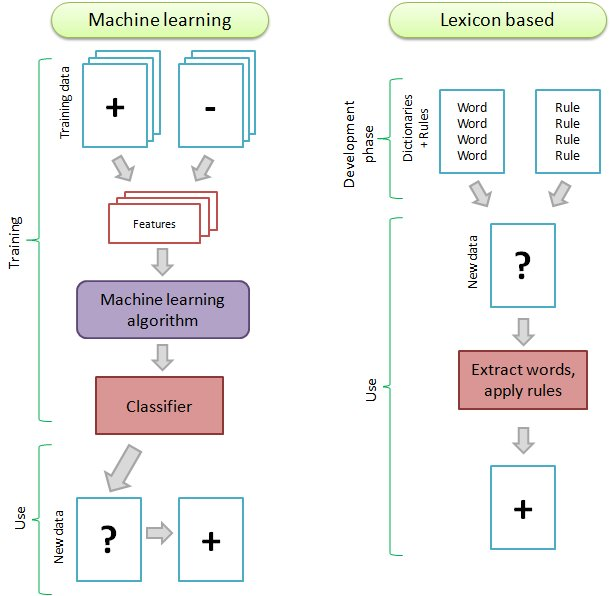
\includegraphics[width=0.7\textwidth]{figures/Machine-learning-and-lexicon-based-approaches-to-sentiment-analysis.jpg}
	\caption{Comparison between machine learning and lexicon-based approaches on sentiment analysis}
	\label{fig:mllbapp}
\end{figure}

\subsubsection{Tokenization}
Given a characters sequence, tokenization is the task of splitting it into pieces, called \textit{tokens}, while also dropping some useless characters like punctuation. Below an example:
\begin{description}
\item Input: Friends, Romans, Countrymen, lend me your ears;
\item Output: ['Friends', 'Romans', 'Countrymen', 'lend', 'me', 'your', 'ears']
\end{description}
It is important to give some definitions \cite{Manning:2008:IIR:1394399}: a token consist in a sequence of characters grouped together in a useful semantic unit, a \textit{type} is the class of all tokens containing the same character sequence, a \textit{term} is a type that is included in a reference dictionary. The major question on tokenization is to select which are the correct tokens to use, for instance, for "\textit{aren't}", which is the more correct tokenization between "\textit{arent}", "\textit{are n't}" or "\textit{aren t}? A simple strategy is to split on all non-alphanumerical characters, but in this case "\textit{aren t}" does not look correct
In general tokenization is language-specific, so every language has its own rules to make a useful tokenization.

\subsubsection{Stopwords removal}
A stopword is a commonly used word, such as "the", "a", "an" or "in" that do not contribute on giving information to a text, so usually are removed. It is possible to achieve language-specific resources to get the list of stopwords for a language. An example of this task is below:
\begin{description}
	\item Input: "This is a sample sentence, showing off the stop words filtration."
	\item Tokenized: ['This', 'is', 'a', 'sample', 'sentence', ',', 'showing', 'off', 'the', 'stop', 'words', 'filtration', '.']
	\item Stopwords removal: ['This', 'sample', 'sentence', ',', 'showing', 'stop', 'words', 'filtration', '.']
\end{description}


\subsubsection{Stemming}
For grammatical reasons, texts use different forms of a word, such as "organize", "organise", "organizing", so it will be useful to refer all these versions to a common one. The goal of stemming is to reduce the set of possible words by transforming all words to their common base form, for instance:
\begin{description}
	\item am, are, is $\Rightarrow$ be
	\item car, cars, car's, cars' $\Rightarrow$ car
\end{description}
The result applied to a complete sentence will be:
\begin{description}
	\item Input: "the boy's cars are different colors"
	\item Output: "the boy car be differ color"
\end{description}
Stemming is usually an heuristic process that respects some linguistic rules that cut off suffixes of the words, and sometimes the affixes. A similar but more complex method is called \textit{lemmatization}. It consists on the same task of stemming, but instead of using heuristics rules, it uses dictionaries and morphological analysis of the words, so it aims to remove inflectional endings only and to return the base or dictionary form, also called \textit{lemma}. An example that shows the difference between stemming and lemmatization can be simply shown on what happens to the word "saw": the stemming returns just "s", whereas lemmatization returns "see".


\subsubsection{Parts Of Speech tagging}
Part of speech tagging (POS tagging) is the process of marking up a word in a text as corresponding to a particular part of speech, based on both its definition and its context. Identifying parts of speech is more complicated than simply mapping words to their part of speech tag, because usually words may have different POS tags with respect to the context, for instance:
\begin{description}
	\item She saw a \textit{bear}.
	\item Your efforts will \textit{bear} fruit.
\end{description}
The same word "bear" has two complete different senses with respect to the context, moreover, it has two different parts of speech: in the first sentence it is a noun, while in the second one it is a verb.\\
To define POS tagging there are essentially two types of taggers. Rule-based taggers use contextual information to assign tags to unknown or ambiguous words. Disambiguation is done by analyzing the linguistic features of the word, its preceding and following ones and other aspects. For instance if the preceding word is an article, the current word must be a noun. Stochastic taggers consist on models that incorporates frequency os probability. In \cite{articlepos} is proposed a comparison between rule-based taggers and stochastic taggers.


\subsubsection{Features extraction and representation}
Especially for machine learning text classification techniques, it is fundamental to translate a document into a numerical vector, in a process called \textit{vectorization}, to be processed by machine learning algorithms. Firstly it is mandatory to define the feature to be vectorized, that represent the document in a multidimensional space. The most implemented feature extraction technique is the \textit{N-Gram}. It consists on extracting a set of n-words which occurs "in that order" in the document. Commonly in a feature representation are used 1-gram (which is just the list of words), 2-gram, 3-gram also together, in order to extract more information in the text.\\
An example of 2-gram:
\begin{description}
	\item Input: "After sleeping for four hours, he decided to sleep for another four."
	\item Output: ['After sleeping', 'sleeping for', 'for four', 'four hours', 'four he' 'he decided', 'decided to', 'to sleep', 'sleep for', 'for another', 'another four']
\end{description}
An example of 3-gram:
\begin{description}
	\item Input: "After sleeping for four hours, he decided to sleep for another four."
	\item Output: ['After sleeping for', 'sleeping for four', 'four hours he', 'hours he decided', 'he decided to', 'to sleep for', 'sleep for another', 'for another four' ]
\end{description}
Once defined the set of features it must be represented in a multidimensional space, where each feature is translated in a number. For this task there are several techniques \cite{DBLP:journals/corr/abs-1904-08067}:
\begin{description}
	\item Bag of Words (BoW) is a simplified version of Term Frequency. It is used in several domains such as computer vision, natural language processing, spam filters as well as text classification. In BoW, a body of text is thought of like a bag of words. These words in a matrix are not sentences which structure sentences and grammar, and the semantic relationships between words and their order is ignored. In this model just the presence of a word matters. The list of used words is processed looking at the entire text in a preliminary phase. Below an example:
	\begin{description}
		\item Input: “As the home to UVA’s recognized undergraduate and graduate degree programs in systems
		engineering. In the UVA Department of Systems and Information Engineering, our students are
		exposed to a wide range of range”
		\item Bag of Words: ['As', 'the', 'home', 'to', 'UVA’s', 'recognized', 'undergraduate', 'and', 'graduate', 'degree', 'program', 'in', 'systems', 'engineering', 'in', 'Department', 'Information', 'students', 'are', 'exposed', 'wide', 'range']
		\item Bag of Features: [1,1,1,3,2,1,2,1,2,3,1,1,1,2,1,1,1,1,1,1]
	\end{description}
	In Bag of Words with a vocabulary of size $|\Sigma|$, every word is encoded in a vector of size $|\Sigma|$, with 1 at index corresponding to the word, and 0 in every other indexes. This model is the cause of issues due to words position in the sentence: the phrases "this is good" and "is this good" have the same BoW representation. Term Frequency is similar to Bag of Words, that consists on counting the number of occurrences of each word instead of just the presence.
	\item Term Frequency-Inverse Document Frequency (TF-IDF) is a method used in conjunction with Term Frequency in order to decrease the effect of commonest words (that usually do not carry information). IDF assigns a higher weight to words with either high or low frequencies term in the document. TF-IDF is the combination of both Term Frequency and Inverse Document Frequency, and it is calculated as
	\[TFIDF(w,d) = TF(w, d) * log(\frac{N}{df(t)})\]
	Where $N$ is the number of documents and $df(t)$ is the number of documents that contain the term $t$. Although TF-IDF overcomes to the issue of commonest words, it keeps suffering the fact that similar words are accounted for similarity since all words are independent one another. 
	\item Other techniques, called Word Embedding, such as Word2Vec \cite{NIPS2013_5021} aim to vectorize words instead of the entire document, but these methods are not used in this work, so I'm not going to describe them.
\end{description}


\subsection{Applications}
Sentiment analysis can be used for a wide range of applications \cite{saifee2013applications}. The most general application is in e-commerce activities, since websites allow users to submit their experience about shopping and product qualities. They provide also summary of the product by assigning rates or scores that customers can easily see. Sentiment analysis helps these websites by converting dissatisfied customers into promoters by analyzing the huge amount of opinions.\\
Voice of Market (VOM) is about determining what customers are feeling about products or services of competitors. Accurate sentiment classification from voice of market involving also temporal information helps in gaining competitive advantage and new product development. Detection of real-time sentiment information may help on planning marketing campaigns and strategies, improving product features in order to satisfy as much customers as possible.\\
Voice of the Customer (VOC) consists on knowing what a customer is saying about a product or service, analyzing his reviews and feedback. VOC is a key element of Customer Experience Management. Extracting such information may help on understand what are the features that customers want on a specific product and what are the ones that do not want, for instance costs.\\
Brand Reputation Management is about managing the reputation in the market. Customers' opinion may enhance or damage brand reputation, so it is important to keep it monitored. Brand information, nowadays, are not just in advertising, public relations, but also in many conversation in online forums or in social media. Sentiment analysis can help brands on knowing how their products, services or the brands themselves are perceived by people and customers.





\section{Sentiment Analysis Datasets}
In this section I'm going to describe some sentiment analysis dataset of different domains. That can be useful in order to compare the proposed ones with the final dataset utilized in this work.

\subsubsection{Pharma \cite{GraBer:2018:ASA:3194658.3194677}}
This dataset provides patients reviews about drugs. Reviews are grouped into the three aspects: benefits, side effects and overall comment. Additionally, ratings are available concerning overall satisfaction as well as a five step side effect rating and five steps effectiveness rating. The data was obtained by crawling online pharmaceutical review sites.\\
The attributes of the dataset are the followings:
\begin{itemize}
	\item \textbf{urlDrugName} (categorical): name of drug 
	\item \textbf{condition} (categorical): name of condition 
	\item \textbf{benefitsReview} (text): patient on benefits 
	\item \textbf{sideEffectsReview} (text): patient on side effects 
	\item \textbf{commentsReview} (text): overall patient comment 
	\item \textbf{rating} (numerical): 10 star patient rating 
	\item \textbf{sideEffects} (categorical): 5 step side effect rating 
	\item \textbf{effectiveness} (categorical): 5 step effectiveness rating
\end{itemize}

Some examples of comments of different sentiments:
\begin{itemize}
	\item \textbf{positive}: "\textit{I was used to having cramps so badly that they would leave me balled up in bed for at least 2 days.  The Ponstel doesn't take the pain away completely, but takes the edge off so much that normal activities were possible. Definitely a miracle medication!!}"
	\item \textbf{neutral}: "\textit{I'm taking Gabapentin to treat nerve disorder. My nerves are inflamed and causes to experience pelvic pain and other pelvic disorders. The Gabapentin sometimes works but I do experience relapse.	For the migraines I find that the 800mg of Ibprofen works better with no side effect for my migraines, but the maxalt has a better track record.}"
	\item \textbf{negative}: "\textit{after taking propecia for over a year, starting when i was 20 years of age my hair continued to thin, and i noticed no significant benefits}"
\end{itemize}

\subsubsection{US Airline \cite{Rane-TSA-Airline}}
Sentiment analysis dataset about problems of major U.S. airline. Tweets acquired from February 2015.

Some meaningful attributes of the dataset are the followings:
\begin{itemize}
	\item airline\_sentiment: sentiment
	\item airline\_sentiment: confidence
	\item airline: subject airline company
	\item name: user's username
	\item text: text of the comment
	\item tweet\_created: timestamp of the tweet
\end{itemize}

Some examples of comments of different sentiments:
\begin{itemize}
	\item \textbf{positive}: "\textit{@VirginAmerica plus you've added commercials to the experience... tacky.}"
	\item \textbf{neutral}: "\textit{@VirginAmerica What @dhepburn said.}"
	\item \textbf{negative}: "\textit{@VirginAmerica it's really aggressive to blast obnoxious "entertainment" in your guests' faces \&amp; they have little recourse}"
\end{itemize}



\subsubsection{IMDB \cite{maas-EtAl:2011:ACL-HLT2011}}
This dataset is a collection of movie reviews, along with their associated binary sentiment polarity labels. It contains balanced positive and negative instances (no neutral class in this dataset). In the collection, no more than 30 reviews are present for any given movie, in order to avoid correlation between reviews of the same movie.

The attributes of the dataset are the followings:
\begin{itemize}
	\item text: text of the review
	\item sentiment: the sentiment of the review
\end{itemize}

Some examples of comments:
\begin{itemize}
	\item \textbf{positive}: "\textit{If you like adult comedy cartoons, like South Park, then this is nearly a similar format about the small adventures of three teenage girls at Bromwell High. Keisha, Natella and Latrina have given exploding sweets and behaved like bitches, I think Keisha is a good leader. There are also small stories going on with the teachers of the school. There's the idiotic principal, Mr. Bip, the nervous Maths teacher and many others. The cast is also fantastic, Lenny Henry's Gina Yashere, EastEnders Chrissie Watts, Tracy-Ann Oberman, Smack The Pony's Doon Mackichan, Dead Ringers' Mark Perry and Blunder's Nina Conti. I didn't know this came from Canada, but it is very good. Very good!}"
	\item \textbf{negative}: "\textit{Story of a man who has unnatural feelings for a pig. Starts out with a opening scene that is a terrific example of absurd comedy. A formal orchestra audience is turned into an insane, violent mob by the crazy chantings of it's singers. Unfortunately it stays absurd the WHOLE time with no general narrative eventually making it just too off putting. Even those from the era should be turned off. The cryptic dialogue would make Shakespeare seem easy to a third grader. On a technical level it's better than you might think with some good cinematography by future great Vilmos Zsigmond. Future stars Sally Kirkland and Frederic Forrest can be seen briefly.}"
\end{itemize}



\vspace{1cm}
In table \ref{table:dataset_statistics} are shown some statistics of proposed datasets.


\begin{table}[ht]
	\centering    
	\begin{tabular}{ | c | c | c | c | c | }
		\hline
		Dataset & Num. instances & Positive & Neutral & Negative\\ 
		\hline
		Pharma & 5009 & 15.6\% & 73.3\% & 11.1\% \\
		U.S. Airline & 14641 & 16.1\% & 21.2\% & 62.7\% \\
		IMDB & 50.000 & 50\% & 0\% & 50\% \\
		\hline
	\end{tabular}
	\captionsetup{justification=centering}
	\caption{Dataset statistics}
	\label{table:dataset_statistics}
\end{table}

The proposed datasets present some differences. 
Since IMDB dataset is thought for sentiment analysis competitions, it is built in order to simplify the classification, setting the data balanced (50\% positives - 50\% negatives). Another characteristic of IMDB is that it does not contain the neutral class: as explained before, product reviews social media generally contain just positives and negatives comments, so in this case the neutral class has been omitted. 
Apart from IMDB, data imbalance issues affect both of the other datasets: Pharma contains lot of neutral comments (73.3\%), while U.S. Airline contains  mostly negative ones (62.7\%). Data imbalance affects real world data, so it is an issue that must be taken in consideration.
An important difference between all of the three datasets consists on the language. While tweets of U.S. Airline are very concise (due to the characters limit), movie reviews are long texts. Long texts may contain sentences that supports different sentiments, for instance an user may express positive sentiment to one aspect of a movie (in case of IMDB), while criticize some other aspects. These cases are more difficult to be handled, since datasets should contain one field for each aspect to be considered, and the corresponding sentiment. In general, the presented cases show a very simple and informal language for what concerns tweets of U.S. Airline, while a long, well expressed and full of information texts for Pharma and IMDB. Lastly, Pharma dataset contains also medical-specific terms.



\section{Supervised Learning}
Since the goal of this work is to apply some machine learning techniques for sentiment analysis, it is needed an introduction to machine learning in a technical way and the most commonly used algorithm utilized in supervised learning, and also in this review.\\
In general, machine learning can be considered a subfield of artificial intelligence, since algorithms in some sense "learn" from data. The core function of machine learning is to automatically find a good predictor based on past experiences. While "learning by memorization" approach is sometimes useful, it lacks an important aspect of learning systems, which is the generalization. To achieve generalization, the learner should scan input data and learn some "rules", so when new data are provided, it can output some meaningful result. While human learners can rely on experience to filter out some meaningless inputs, on machine learning data must be well defined, and based on principles that protect the learner from reaching senseless conclusions.\\
Before going in detail, it is important to understand why we need machine learning. There are tasks that humans and animals do everyday, where it is too difficult to extract a well defined program, for instance driving, speech recognition, image understanding, or tasks that humans cannot do, for instance analysis and understanding of large and complex data sets. Other tasks need adaptivity on input data, feature that programmed tools cannot achieve, for instance handwritten text decoding, or the just described sentiment analysis.\\
Machine learning is, in general, a wide domain, so it is branched in several subdomains with respect to the different approaches and goals. Learning can be divided in supervised and unsupervised, depending on the fact that ground truth examples are provided or not. In unsupervised learning, clustering and pattern recognition are the most famous techniques. Supervised learning, instead, can be viewed as learning from examples, where training samples contain information that test ones do not. From here on I will focus on just supervised learning.\\

\subsection{Supervised Learning Model Definition}
The fist step is to define a statistical learning model \cite{Shalev-Shwartz:2014:UML:2621980}.
\begin{itemize}
	\item \textbf{Learner's input}: 
	\begin{itemize}
		\item \textbf{Domain set}: an arbitrary set $X$ of samples that we wish to label. Usually samples, also called \textit{instances}, are represented by vectors of \textit{features}.
		\item \textbf{Label set}: the set $\mathcal{Y}$ of all possible labels, for instance $\mathcal{Y}=\{0,1\}$
		\item \textbf{Training data}: the set $S=((x_1,y_1), \dots, (x_n,y_n))$ finite sequence of labeled points on $\mathcal{X} \times \mathcal{Y}$. That is the input provided to the learner.
	\end{itemize}

	\item \textbf{Learner's output}: the learner is requested to output a \textit{prediction rule} $h: \mathcal{X} \rightarrow \mathcal{Y}$, called also \textit{hypothesis} or \textit{classifier}. It can be used to predict labels of new points.
	
	\item \textbf{Data generation model}: we assume that instances are generated by some probability distribution $D$ over $X$, that represents the environment. It is important that the learner should not know anything about the distribution. We assume also that there is a correct labeling function $f: \mathcal{X} \rightarrow \mathcal{Y}$, and that $f(x_i) = y_i, \forall i$, almost initially. The labeling function is unknown, since it is what the learner aims to find. Summarizing, each pais of $S$ is sampled according to $D$ and then labeled by $f$.
	
	\item  \textbf{Measure of success}: we define the \textit{error of the classifier} the probability that it does not predict the correct label of a point generated according to the generative distribution. Formally, it is defined as:
	\[L_{D,f}(h) \stackrel{\text{def}}{=} P_{x \sim D}(h(x) \neq f(x)) \]
	That is, given a predictor $h$, the probability that randomly chosen an observation $x$ according to $D$, we have that $h(x) \neq f(x)$.\\
	$L_{(D,f)}(h)$ is called \textit{generalization error}, or \textit{true error} of $h$.
	
\end{itemize}


\subsection{Empirical Risk Minimization}
The learner that receives in input a training set S, outputs an hypothesis $h_s : x \rightarrow Y$. The algorithm searches the hypothesis $h_s$ that minimizes the error, but since both $D$ and $f$ are not known, it minimizes the so called \textit{training error} $L_s$ defined as:
\[ L_s(h) \stackrel{\text{def}}{=} \frac{|\{i \in [m] : h(h_i) \neq y_i\}|}{m} \]
for $[m] = {1, \dots, m}$. Empirical Risk Minimization (ERM) is the task of searching a predictor that minimizes $L_s(h)$ that makes sense, since the only information available to the learner is just the training set $S$ (that should be a snapshot of the world), moreover, since $D$ and $f$ are unknown, minimizing the true error is not possible.\\
ERM rule, however, may have the side effect that learns "too well" training data, that does not work well on new data from $D$. This effect is called \textit{overfitting}, and a common solution to prevent it, is searching $h$ in a restricted set of predictors. In this way, ERM rule can be written as:
\[hs \in argmin_{h \in H} L_s(h)\]
By restricting on a finite set of hypotheses $H$, we \textit{bias} the learner, since we cannot guarantee that the algorithm picks the optimal one.\\

ERM rule depends on training set $S$, so a general assumption is to consider elements in $S$, independently and identically distributed according to the distribution $D$. However, picking a restricted number of samples, it is possible that those data are not \textit{representative} of the distribution, and the learner may be affected by this issue. Furthermore, it is more realistic to not assume that labels are fully determined by features on input data. Saying $\delta$ the probability that the training set is not representative, and $\epsilon$ an \textit{accuracy parameter}, it is possible to interpret $(1-\delta)$ as a \textit{confidence parameter}, and the event $L_{(D,f)}(h_s) > \epsilon$ a failure of the learner.\\
After these assumptions, the goal of the learner is to find a predictor that is probably approximately correct, formally an hypothesis $h_s$ that with probability $> (1-\delta)$ (that determines how confident is the solution), upper bounds the generalization error $L_{(D,f)}(h_s) < \epsilon$ (how well the predictor has learned). Since $D$ and $f$ are still not known, the learner tries to find the optimal hypothesis by minimizing the empirical risk.\\

\subsubsection{Machine Learning Tasks}
The model discussed so far can be applied in multiple machine learning tasks.
\begin{itemize}
	\item \textbf{Classification}. It is the task of predicting a discrete and finite set of labels. Such algorithms have access to a set of correctly classified samples, and on the base of these instances, learns a predictor that taken a new instance, it predicts its own class. Classification ca be binary or multiclass, depending on the size of the possible set of labels. This work is focused on this task, more precisely on both binary and muticlass classification.
	\item \textbf{Regression}. It is the task of fining some simple patterns on data that a re functional dependencies beyween the sets $\mathcal{X}$ and $\mathcal{Y}$.
\end{itemize}

A supervised learning task can be seen as an optimization problem that aims to minimize a \textit{loss function}. Introducing some formalism, a loss function $\ell$ is a function from $\mathcal{X} \times \mathcal{Y}$ to the set of non negative real numbers
\[\ell: \mathcal{X} \times \mathcal{Y} \rightarrow \mathbb{R}_+\]
Saying $z$ belonging to $\mathcal{X} \times \mathcal{Y}$, the generalization error becomes:
\[L_D(h) \stackrel{\text{def}}{=} \mathbb{E}_{z \sim D}[\ell (h,z)]\]
While the empirical risk becomes:
\[L_s(h)\stackrel{\text{def}}{=} \frac{1}{m} \sum_{i=1}^{m} \ell (h, z_i)\]

The loss function $\ell$ is characteristic of the learning task: in binary and multiclass classification, the so called 0-1 loss is the correct choice:
\[\ell_{0-1}(h, (x,y)) \stackrel{\text{def}}{=} 
	\begin{cases}
		0 \quad \textrm{if} \quad  h(x) = y\\
		1 \quad \textrm{if} \quad  h(x) \neq y
	\end{cases}\]
That intuitively counts the number of misclassified samples. While in regression tasks, the squared loss is a better choice:
\[\ell_{sq}(h,(x,y)) \stackrel{\text{def}}{=} (h(x)-y)^2\]

% TODO eventualmente parlare del no free lunch theorem



\subsection{Model Selection and Validation}
Suppose we are facing a classification problem. As explained so far, the common approach is applying the ERM rule on a training set $S$ restricting to a finite set of hypotheses $H$. However, we want to try different algorithms (or same algorithm with different parameters) on the same training set, and finally select the best predictor. In this way we need new data in order to evaluate the performance of the algorithms, so usually the approach is the following: the training set is splitted in two parts, training and validation sets. The first set is used to train the whole set of algorithms, obtaining the set $H = {h_1, \dots, h_r}$ of best predictors, then these hypotheses are tested on the validation set, and only the hypothesis that reaches the minor loss is picked (actually we apply the ERM rule on $H$).

In Figure \ref{fig:valid-curve} it is shown the usual behavior in validation: training error is monotonically decreasing, because on growing the model complexity, the data are more well fitted. The validation error, instead, at some point starts increasing, that is symptom of overfitting. In this way, the predictor that should be chosen on validation is the one with complexity equal to the point on which the validation curve starts increasing, limiting both overfitting and underfitting.
\begin{figure}
	\centering
	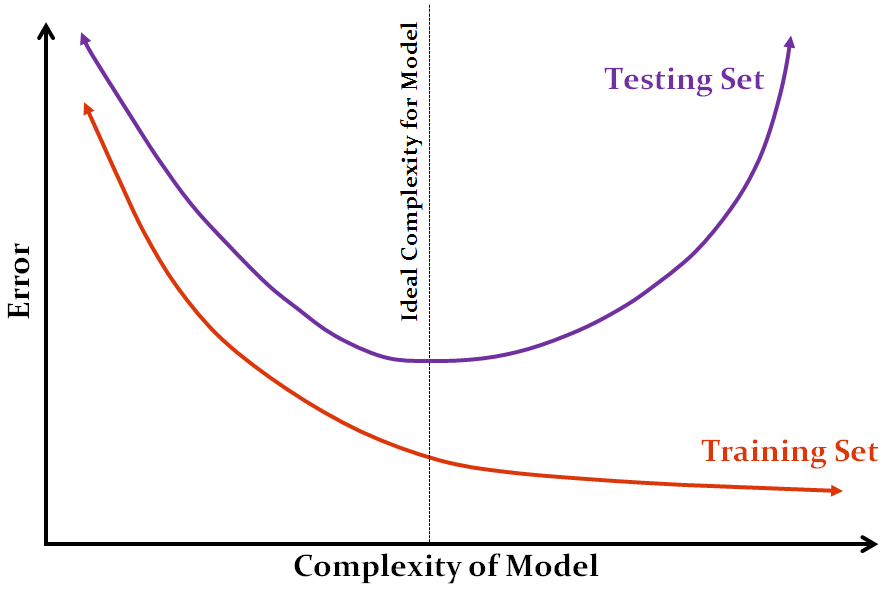
\includegraphics[width=0.7\textwidth]{figures/validation-lern-curve.png}
	\caption{Learning curve for training and validation}
	\label{fig:valid-curve}
\end{figure}

In practical problems, the dataset is splitted into three subsets: the training set is used to train the learning algorithms, the validation set is used to select the best learned model, and the test set is used to estimate the true error. This last set cannot be used in the learning process, otherwise it can bias the final result, so it must be used only once. If the learning fails, new data must be used for test the final model.


\subsubsection{K-Fold Cross Validation}
Sometimes data are not plenty, so test-validation split may reduce too much the training set size, so a common approach is the so called \textit{k-fold cross validation} \cite{Refaeilzadeh2009}. In this technique, data is partitioned in $k$ subsets of equal size called \textit{folds}, usually respecting the labels distribution in a process called \textit{stratification}. Then, for $k$ iterations, the learning algorithm is trained with $k-1$ folds, and validated using the last one, as shown in Figure \ref{fig:kfold}. Finally, the score is calculated as the average of the $k$ scores obtained with the $k$ validation tests. 

\begin{figure}[ht]
	\centering
	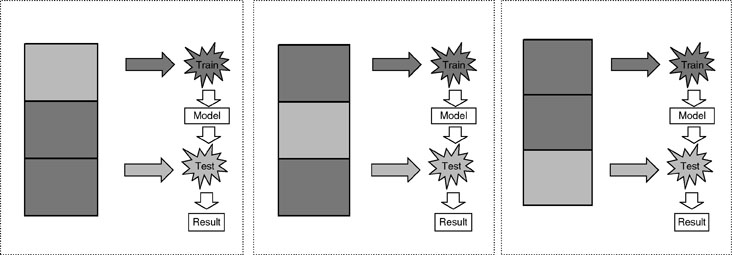
\includegraphics[width=1\textwidth]{figures/kfold.jpg}
	\caption{Example of k-fold cross validation with k=3}
	\label{fig:kfold}
\end{figure}


\subsection{Linear Models}
One of the most important and commonly used hypotheses class is the one of \textit{linear predictors}. Since this class is used also in this work, it deserves a dedicated focus.\\
Define the class of affine functions as:
\[ L_d = \{h_{\textbf{w},b} : \mathbf{w} \in \mathbb{R}^d, b \in \mathbb{R} \} \]
where
\[ h_{\mathbf{w}, b}(\mathbf{x}) = \langle \mathbf{w},\mathbf{x} \rangle + b = \left( \sum_{i=1}^{d} w_i x_i \right) + b \]

$L_d$ is a set of functions, parameterized by $\mathbf{w} \in \mathbb{R}^d$ and $b \in \mathbb{R}$, that take in input a vector $x \in \mathbb{R}^d$ and outputs $\langle \textbf{w},\textbf{x} \rangle + b$, which is a scalar.
The different hypotheses classes are compositions of a function $\Phi : \mathbb{R} \rightarrow \mathcal{Y}$ on $L_d$, for instance in binary classification the function $\Phi$ can be chosen as the sign function.\\
Usually the parameter $b$ is incorporated into $\mathbf{w}$ adding one extra coordinate equal to 1 as follows:\\
let $w'=(b, w_1, \dots , w_d) \in \mathbb{R}^{d+1}$ and let $x'=(b, x_1, \dots , x_d) \in \mathbb{R}^{d+1}$.\\
Therefore, \\
$h_{\mathbf{w},b}(\mathbf{x}) = \langle \mathbf{w},\mathbf{x} \rangle + b = \langle \mathbf{w'},\mathbf{x'} \rangle$
so in general the parameter $b$ is omitted because included in $\mathbf{w}$. It follows that each affine function can be thought as a homogeneous linear function in an upper dimension, with a coordinate equal to 1.\\
The class used for binary classification is the \textit{halfspaces class}. It is made by the composition of the class of linear functions $L_d$ with the sign function, so $\mathcal{X}=\mathbb{R}^d$ and $\mathcal{Y}=\{-1,1\}$.
\[ HS_d = sign \circ L_d = \{ sign( h_{\mathbf{w},b}(\mathbf{x}) ) : \mathbf{x} \in \mathbb{R}^d, h_{\mathbf{w},b}(\mathbf{x}) \in L_d \} \]
Each hypothesis forms an hyperplane that is perpendicular to $\mathbf{w}$, and intersects the vertical axis in $(0, -\frac{b}{w_2})$. The instances that are "above" the hyperplane, which means on the same direction of $\mathbf{w}$, are labeled positively, while the others negatively, as shown in Figure \ref{fig:halfspace}.

\begin{figure}[ht]
	\centering
	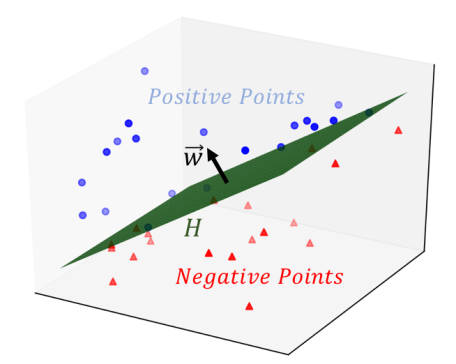
\includegraphics[width=0.6\textwidth]{figures/halfspace.png}
	\caption{Halfspace in $\mathbb{R}^3$}
	\label{fig:halfspace}
\end{figure}










\subsection{Regularization}
In common machine learning problems, it is important to be on guard against overfitting. In some cases a philosophical solution comes from the \textit{Occam's Razor}, which states that from a pool of solutions, it is better to choose the simplest one, on the basis that they are capturing more fundamental aspects. \textit{Regularization} is an application of this principle to ERM: instead of searching the model that best fits the training data, a penalty based on the model complexity is added. In fact, in general, algorithms tend to overfit the training data, learning a model that is more complex, so adding a penalty on the optimization function, makes the learner more \textit{stable}, that also generalize better \cite{stability_generalization}.
The ERM rule becomes:
\[argmin_\mathbf{w} (L_s(\mathbf{w}) + R(\mathbf{w}))\]
Where $R(\mathbf{w}))$ is a regularization function $R: \mathbb{R}^d \rightarrow \mathbb{R} $. This approach is called \textit{Regularized Loss Minimization} (RLM). Intuitively, the model complexity is measured by the value of the regularization function, and the algorithm balances between low empirical risk and simpler hypotheses.\\
Some common regularization functions are the followings:
\begin{itemize}
	\item \textbf{L1 Regularization}: the regularization function is
	\[ R(\textbf{w}) = \lambda \sum_{i=1}^{m} |w_i| \]
	\item \textbf{L2 Regularization}: the regularization function is
	\[ R(\textbf{w}) = \lambda \sum_{i=1}^{m} (w_i)^2 \]
\end{itemize}

Writing the expected risk of a learning algorithm as
\[ \mathbf{E}_S[L_D(A(S))] = \mathbf{E}_S[L_S(A(S))] + \mathbf{E}_S[L_D(A(S)) - L_S(A(S))] \]
it is shown that it is composed by two terms: the first one describes how well the algorithm fits the training data, and increases with $\lambda$, while the second one reflects just the difference between the true risk and the empirical risk. This second term can be seen as the stability of the learner, and decreases with $\lambda$. We are facing a tradeoff between fitting and stability that reflects on the choice of the parameter $\lambda$.



\subsection{Gradient Descent}

The goal of a machine learning task is to minimize the risk function $L_d(h)$. It is not possible to minimize it directly, since it depends on the unknown distribution $D$, so another approach is mandatory. In general there are multiple possible approaches, but the most used derives from the \textit{Gradient Descent} (GD) \cite{article-gs-sgd}. \\
Recall that the gradient $\nabla f(\mathbf{w})$ of a differentiable function $f: \mathbb{R}^d \rightarrow \mathbb{R}$ is the vector  $\nabla f(\mathbf{w}) = \left( \frac{\partial f(\mathbf{w})}{\partial w_1}, \dots, \frac{\partial f(\mathbf{w})}{\partial w_d} \right)$, that points to the direction of maximum growth of the function. Gradient descent is an iterative algorithm that starts from a initial point $\mathbf{w}^{(0)}$, and at each iteration $t$ updates the point by "moving" a step in the opposite direction of the gradient, as
\[ \mathbf{w}^{(t+1)} = \mathbf{w}^{(t)} - \eta \nabla f(\mathbf{w}^{(t)}) \]
where $\eta > 0$ is a parameter that intuitively defines the length of the step. After $T$ iterations of the algorithm, the value of the function should converge to a value $\mathbf(w)^{(T)}$, which is the supposed minimum (since it is an heuristic, the result is not guaranteed to be the absolute minimum, but just a local minimum). The final result can be either the last vector found $\mathbf{w}^{(T)}$, the best performing $argmin_{t \in T} f(\mathbf{w}^{(t)})$, or the average $\mathbf{\bar{w}} = \frac{1}{T} \sum_{i=1}^{T} \mathbf{w}^{(t)}$ (preferred in the case of non differentiable functions). The pseudocode of GD is shown in Algorithm \ref{alg:GD}.

\begin{algorithm}
\caption{Gradient Descent}\label{alg:GD}
\begin{algorithmic}[1]
	\State \textbf{parameters}: scalar $\eta > 0$, integer $T>0$
	\State \textbf{initialize}: $\mathbf{w}^{(1)} = \mathbf{0}$
	
	\For $t = 1, 2, \dots , T$
	\State $\mathbf{w}^{(t+1)} = \mathbf{w}^{(t)} - \eta \nabla f(\mathbf{w}^{(t)})$
	\EndFor
	
	\State \textbf{output}: $\mathbf{\bar{w}} = \frac{1}{T} \sum_{i=1}^{T} \mathbf{w}^{(t)}$
\end{algorithmic}
\end{algorithm}


However, in Gradient Descent it is required to know the exact gradient of the function, which is unfeasible especially when working on large sets of data, so an approximation may be useful as well. \textit{Stochastic Gradient Descent} (SGD) requires that the expected value of the update direction is equal to the gradient direction, which is a great advantage in terms of calculations, since it requires less points to be calculated.b The pseudocode of SGD is shown in Algorithm \ref{alg:SGD}.

\begin{algorithm}
	\caption{Stochastic Gradient Descent}\label{alg:SGD}
	\begin{algorithmic}[1]
		\State \textbf{parameters}: scalar $\eta > 0$, integer $T>0$
		\State \textbf{initialize}: $\mathbf{w}^{(1)} = \mathbf{0}$
		
		\For $t = 1, 2, \dots , T$
		\State choose $\mathbf{v_t}$ at random from a distribution such that $\mathbb{E}[\mathbf{v_t} | \mathbf{w}^{(t)}] \in \partial f(\mathbf{w}^{(t)})$
		\State $\mathbf{w}^{(t+1)} = \mathbf{w}^{(t)} - \eta \nabla \mathbf{v_t}$
		\EndFor
		
		\State \textbf{output}: $\mathbf{\bar{w}} = \frac{1}{T} \sum_{i=1}^{T} \mathbf{w}^{(t)}$
	\end{algorithmic}
\end{algorithm}

A visual demonstration of the behavior of both Gradient Descent and Stochastic Gradient Descent is shown in Figure \ref{fig:gd-sgd}. It is shown that SGD to reach the minimum, takes more steps in a direction that is not exactly the gradient direction, but only on the average.


\begin{figure}[ht]
	\centering
	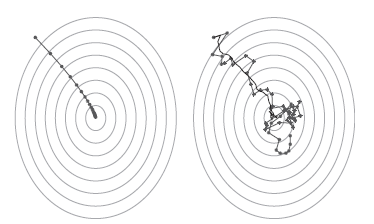
\includegraphics[width=0.8\textwidth]{figures/gd-sgd.png}
	\caption{Behavior of Gradient Descent (left) and Sochastic Gradient Descent (right).}
	\label{fig:gd-sgd}
\end{figure}


\subsection{Feature Selection}

As early explained, supervised learning is based on finding a proper function that joins the input vectors of features $\mathcal{X}$ with their label $\mathcal{Y}$. Sometimes, the output $\mathcal{Y}$ does not depend by all features $(X_1, \dots, X_d)$, instead, it is decided by a subset of them $(X_{(1)}, \dots, X_{(r)})$, with $r<d$. With sufficient data and time, it is fine to use all input features for learning a classification algorithm (including also those irrelevant), but in practice there are motivations for that it is preferable to select only relevant ones.\\

\begin{itemize}
	\item The irrelevant features will induce great computational cost. 
	\item The irrelevant features may lead to overfitting, for instance if in sentiment analysis the name of the person for which it is going to classify the comment is included in the features set, then the classification algorithm may depend on this (which obviously is a mistake).
	\item Since the goal of supervised classification is to estimate a function with respect to the input features, it is reasonable to ignore features with low impact on the decision making, in order to keep the model as simple as possible.
\end{itemize}

The feature selection problem has been studied for many years, in fact many solutions are proposed for machine learning tasks. Below are presented some heuristic feature selection procedures that have been implemented in this work.


\subsubsection{Feature Selection for Linear SVM}

In linear classifiers, the outcome of a sample vector $x = (x_1, \dots, x_d)$ is calculated as $y=sign(\mathbf{w}^T\mathbf{x})$. In \cite{Brank2002FeatureSU} it is explained a feature selection method that uses the intuitive fact that weights with small absolute value $|w_j|$ does not contribute much on the decision ov the value $y$. This means that those features are not relevant on the final decision, so they could be discarded. This situation is valid also for SVM with linear kernel, while for other non-linear kernels it is not applicable.\\
The described strategy involves the linear SVM classifier, and it is the following:
\begin{itemize}
	\item Train the classifier with training data;
	\item Eliminate the features whose weight is close to zero, formally setting a threshold $T$, just keep the features $\{w_i : i \in [d], |w_i| > T\}$;
	\item Finally, re-train the model using just the selected features.
\end{itemize}

\subsubsection{Feature Selection $L_1$ norm Regularization}

In regularization, it is optimize a function composed by both empirical risk, and a regularization function. In case of $L_1$ norm regularization, the term
\[ \lambda \sum_{i = 1}^{d} |w_i| \]
especially when $\lambda$ is large, forces some of the weights $w_i$ to be exactly equal to zero \cite{article-lasso}. A typical behavior of the values of the weights with $L_1$ norm regularization is shown in Figure \ref{fig:lasso}.

\begin{figure}[ht]
	\centering
	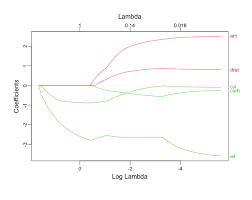
\includegraphics[width=0.7\textwidth]{figures/lasso.png}
	\caption{Behavior of weights on $L_1$ norm regularization on with respect to $\lambda$.}
	\label{fig:lasso}
\end{figure}

It is possible to see that $L_1$ norm regularization selects automatically some weights to be nonzero, while sets zero the others. In this situation, the features to be kept are obviously the one with nonzero values. The strategy is the same as previously mentioned:

\begin{itemize}
	\item Train the classifier with training data;
	\item Eliminate the features whose weight is zero (or close to);
	\item Finally, re-train the model using just the selected features.
\end{itemize}



\subsubsection{Information Gain Feature Selection}

Intuitively, \textit{Information Gain} (IG) measures the amount of information in bits about the class prediction, if the only information available is the presence of a feature and the corresponding class distribution \cite{Roobaert_chapter22}.\\
Given a random variable $X$, the following definitions comes from Shannon's Information theory \cite{Shannon1948}:
\begin{itemize}
	\item The Information associated to an event $x$ from the distribution $X$ is
	\[ I(x) = \log_2 \frac{1}{\mathbb{P}_X(x)} = - \log_2 \mathbb{P}_X(x) \]
	\item The Entropy of a random variable $X$ is the average amount of information of the possible events
	\[ H(X) = - \sum_{x \in X} \mathbb{P}_X(x) \log_2 \mathbb{P}_X(x) \]
\end{itemize}

Both Information and Entropy are pure numbers, but "measured" in \textit{bits}.\\
Concretely, information gain measures the expected reduction in entropy by choosing a given feature. The information gain of a training set $S$ with respect to a feature $i \in [d]$ is calculated as:
\[ IG(S, i) = H(S) - \sum_{v \in values(X_i)} \mathbb{P}(X_i = v) H(S_{X_i=v}) \]
Where $X_i$ is the set of values of the feature $i$, and $S_{X_i=v}$ is the training set restricted to the samples where $X_i=v$.\\
Feature selection using information gain works as follows: given the training dataset $S$, the information gain score is calculated for each feature $X_i$. Next, all scores are sorted in a ranking, then the most important features are selected. The selection can be done either by choosing a threshold on the information gain, or by choosing the size of the set of the selected features.\\



In the followings sections are presented some of the most used algorithms for binary classification, that are also exploited in this work.


\subsection{Logistic Regression}

\textit{Logistic Regression} is a model that analyzes the relationships between multiple independent variables, and a categorical dependent variable, namely between the features and the labels in case of a supervised classification task \cite{article-logreg}.\\
In the context of linear models, it was described the class of hyperplanes, which is a set of functions from $\mathbb{R}^d$ to $\{0,1\}$. However, in some cases it may be useful to have a measure of confidence about the prediction. Logistic Regression provides that information by defining the probability that the label of an input instance $\mathbf{x}$ is $1$. Calling $\mathbb{P}_\mathbf{w}[\mathcal{Y} | \mathcal{X}]$ that conditional probability to get the label $\mathcal{Y}$ given the instance $X$, under the estimator with parameter $\mathbf{w}$. Statistical theory suggest that the probabilistic classifier should be learned from the training set $S$ using the MLE estimator as:
\[ \hat{\mathbf{w}}_{MSE} = argmax_\mathbf{w} \quad \mathbb{P}_\mathbf{w}[y_1 | x_1], \dots , \mathbb{P}_\mathbf{w}[y_n | x_n] \]

In Logistic Regression the conditional probability $\mathbb{P}_\mathbf{w}[\mathcal{Y} | \mathcal{X}]$ is expressed as:
\[ \mathbb{P}_\mathbf{w}[\mathcal{Y}=y | \mathcal{X}=x] = \frac{1}{1 + e^{y \langle \mathbf{w}, \mathbf{x} \rangle}} \]
where $y$ can be either $-1$ or $1$. This result is obtained by the composition of the prediction of the classifier $y = \langle \mathbf{w}, \mathbf{x} \rangle$ (which has no bounds on the values) with the sigmoid function

\[ sig(t) = \frac{1}{1 + e^{-t}} \]
which is shown in Figure \ref{fig:sigmoid}.

\begin{figure}[ht]
	\centering
	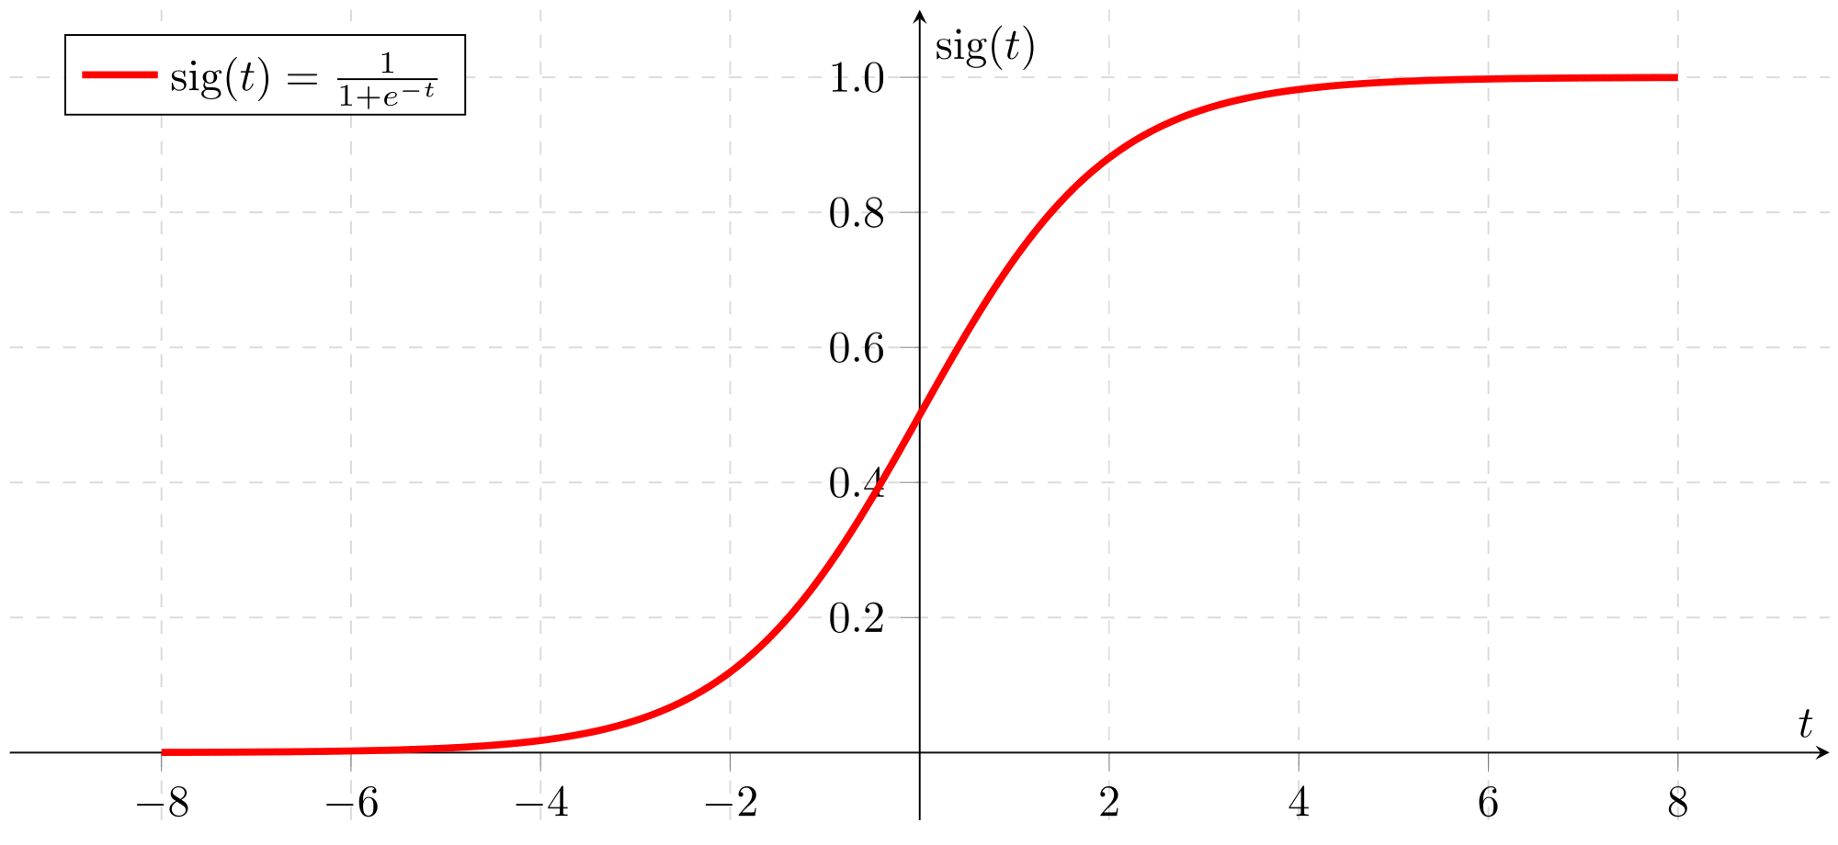
\includegraphics[width=0.8\textwidth]{figures/sigmoid.png}
	\caption{Sigmoid function.}
	\label{fig:sigmoid}
\end{figure}

The hypotheses class is therefore
\[ H_{logreg} = sig \circ L_d = \{ sig(\langle \mathbf{w}, \mathbf{x} \rangle) : \mathbf{x}, \mathbf{w} \in \mathbb{R}^d \} \]

An interpretation of the formulas may be useful to understand. As long the value $\langle \mathbf{w}, \mathbf{x} \rangle$ is large, the predictor can be considered sure about the prediction (the value is far from the separating hyperplane). Contrary, if the value $\langle \mathbf{w}, \mathbf{x} \rangle$ is low, it means that $\mathbf{x}$ falls nearby the separating hyperplane, so the prediction may be less confident. Applying the prediction value to the sigmoid function, as long the value is large, the result is getting closer to $1$, while when the prediction value becomes negative, the final value is getting closer to $0$.
Therefore, the value obtained by the sigmoid can be viewed as the probability that the input value $\mathbf{x}$ has label $1$.\\
Summarizing all the concepts, the final goal is to have the value $y \langle \mathbf{w}, \mathbf{x} \rangle > 0$ for each $(x, y) \in S$ (or more conveniently $\gg 0$). Recalling the Maximum Likelyhood Estimator solution as

\begin{align*}
 \hat{\mathbf{w}}_{MSE} &= argmax_{\mathbf{w} \in \mathbb{R}^d} \quad \mathbb{P}_\mathbf{w}[\mathcal{Y} | \mathcal{X}]	\\
 						&= argmax_{\mathbf{w} \in \mathbb{R}^d} \quad \prod_{i=1}^{n} \frac{1}{1 + e^{-y_i \langle \mathbf{w}, \mathbf{x_i} \rangle}}	\\
 						&= argmin_{\mathbf{w} \in \mathbb{R}^d} \quad \sum_{i=1}^{n} log(1 + e^{-y_i \langle \mathbf{w}, \mathbf{x_i} \rangle})
\end{align*}

which derives the final optimization problem as:
\[ argmin_{\mathbf{w} \in \mathbb{R}^d} \quad \sum_{i=1}^{n} log(1 + e^{-y_i \langle \mathbf{w}, \mathbf{x_i} \rangle}) \]

The same result can be reached following the ERM rule by setting the loss function increasing with the probability that the estimator is wrong, formally defining
\[ \ell (h_\mathbf{w}, (\mathbf{x}, y)) = log(1 + e^{-y \langle \mathbf{w}, \mathbf{x} \rangle}) \]
The associated ERM problem becomes
\[ argmin_{\mathbf{w} \in \mathbb{R}^d} \quad \frac{1}{n} \sum_{i=1}^{n} log(1 + e^{-y_i \langle \mathbf{w}, \mathbf{x_i} \rangle}) \]



\subsection{SVM}

In context of binary classification, \textit{Support Vector Machines} became one of the most popular classification methods \cite{article-svm}. SVM is based on the hypotheses class of hyperspaces, already described, and the main concept is to find the hyperplane that best classifies the training data.

\subsubsection{Hard-SVM}

Suppose that training data are linearly separable, formally
\[ \forall i \in [m], y_i (\langle \mathbf{w}, \mathbf{x}_i \rangle) > 0 \]
intuitively, there exists an hyperplane that classifies correctly every instance ot the training set, like the one shown in Figure \ref{fig:linearly-separable}

\begin{figure}[ht]
	\centering
	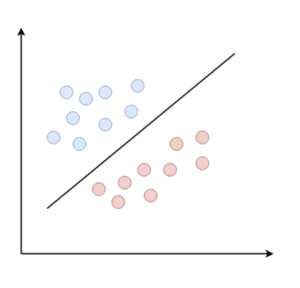
\includegraphics[width=0.5\textwidth]{figures/linearly-separable.png}
	\caption{Example of linearly separable set.}
	\label{fig:linearly-separable}
\end{figure}

Given a set of possible separating hyperplanes, it is intuitively better to prefer the one with largest \textit{margin}. The margin of an hyperplane with respect to a training set is defined to be the minimal distance between the hyperplane and a point of the set, formally
\[ min_{i \in [m]} | \langle \mathbf{w}, \mathbf{x}_i \rangle + b | \]
Therefore, the Hard-SVM rule, which finds the largest margin in linearly separable case is:
\[ argmax_{(\mathbf{w}, b) : \left\lVert \mathbf{w} \right\rVert = 1} min_{i \in [m]} \quad | \langle \mathbf{w}, \mathbf{x}_i \rangle + b | \quad s.t. \quad \forall i \in [m], y_i (\langle \mathbf{w}, \mathbf{x}_i \rangle) > 0 \]
Or another equivalent formulation as a quadratic optimization problem is
\[ (\mathbf{w}_0, b_0) = argmin_{(\mathbf{w}, b)} \left\lVert \mathbf{w} \right\rVert ^2 \quad s.t. \quad \forall i \in [m], y_i (\langle \mathbf{w}, \mathbf{x}_i \rangle) \ge 1 \]
The output should be $\hat{\mathbf{w}} = \frac{\mathbf{w}_0}{\left\lVert \mathbf{w}_0 \right\rVert}$, $\hat{b} = \frac{b_0}{\left\lVert \mathbf{w}_0 \right\rVert}$.

The result of the Hard-SVM optimization problem is shown in Figure \ref{fig:hard-svm}.

\begin{figure}[ht]
	\centering
	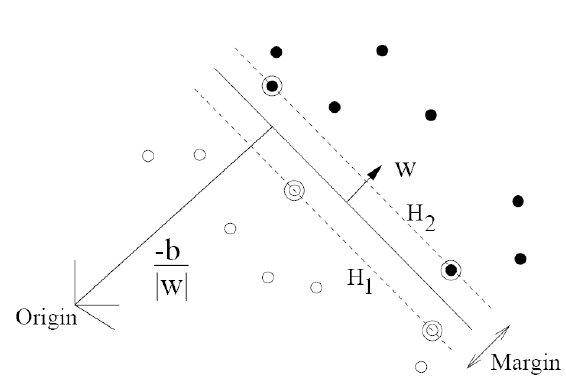
\includegraphics[width=0.6\textwidth]{figures/hard-svm.jpg}
	\caption{Hard-SVM solution.}
	\label{fig:hard-svm}
\end{figure}

The points at minimum distance from the hyperplane are called \textit{Support Vectors}.

\subsubsection{Soft-SVM}

The Hard-SVM formulation supposes that data are linearly separable, however in usual cases, data are not. To handle this situation, Soft-SVM model permits to some points to fall in the wrong side of the hyperplane, but adding a penalty on the objective function represented by \textit{slack} variables $\xi _i$ , that control how far from the wrong side the point $\mathbf{x}_i$ is. The optimization problem becomes
\[ argmin_{(\mathbf{w}, b)} \frac{1}{2} \left\lVert \mathbf{w} \right\rVert ^2 + C \sum_{i=1}^{m} \xi_i \quad s.t. \quad \forall i \in [m], y_i (\langle \mathbf{w}, \mathbf{x}_i \rangle) \ge 1 - \xi_i , \xi \ge 0  \]
The parameter $C$ is a regularization parameter, that controls the trade-off between margin's size and the training errors. 

\begin{figure}[ht]
	\centering
	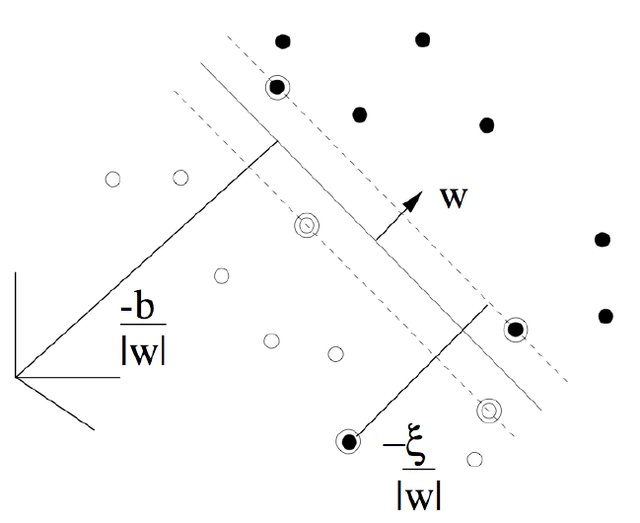
\includegraphics[width=0.6\textwidth]{figures/soft-svm.jpg}
	\caption{Soft-SVM solution.}% Misclassified points highlighted with arrows.}
	\label{fig:soft-svm}
\end{figure}

Solving both the Hard-SVM and Soft-SVM optimization problems is quite hard, due to the complicated constraints \cite{Bottou06supportvector}. The mathematical tool for simplify the problem is the Lagrangian duality theory \cite{1886529043}.\\
From theory, calling $\mathbf{w}_0$ the solution of Hard-SVM problem, and calling $I = {i : |\langle \mathbf{w}_0, \mathbf{x}_i \rangle| = 1}$ (the set of indices that defines the support vectors), then there exist coefficients $\alpha_1, \dots, \alpha_m$ such that
\[ \mathbf{w}_0 = \sum_{i \in [I]} \alpha _i \mathbf{x}_i \]
The same result is valid also for Soft-SVM problem. The Lagrangian duality theory leads to solving the Hard-SVM dual optimization problem
\[ max_{\mathbf{\alpha} \in \mathbb{R}^m} \left( \sum_{i=1}^{m} \alpha_i -\frac{1}{2} \sum_{i=1}^{m} \sum_{i=1}^{m} \alpha_i \alpha_j y_i y_j \langle \mathbf{x}_i, \mathbf{x}_j \rangle \right) \]
subject to
\[ \forall i, \quad \alpha_i \ge 0 , \quad \sum_i y_i \alpha_i = 0 \]
and the Soft-SVM dual optimization problem
\[ max_{\mathbf{\alpha} \in \mathbb{R}^m} \left( \sum_{i=1}^{m} \alpha_i -\frac{1}{2} \sum_{i=1}^{m} \sum_{i=1}^{m} \alpha_i \alpha_j y_i y_j \langle \mathbf{x}_i, \mathbf{x}_j \rangle \right) \]
subject to
\[ \forall i, \quad 0 \le \alpha_i \le C , \quad \sum_i y_i \alpha_i = 0 \]
The resulted dual problems are much simpler, since the constraints are less complicate.\\

\subsubsection{Kernels}

Sometimes points in the training set are far from being linearly separable, like the one in Figure \ref{fig:kernel}. This is because the expressiveness of the halfspaces class is limited. However, it is possible to map the original instance space into another space (possibly of a higher dimension), and then learn a halfspace in that space.

\begin{figure}[ht]
	\centering
	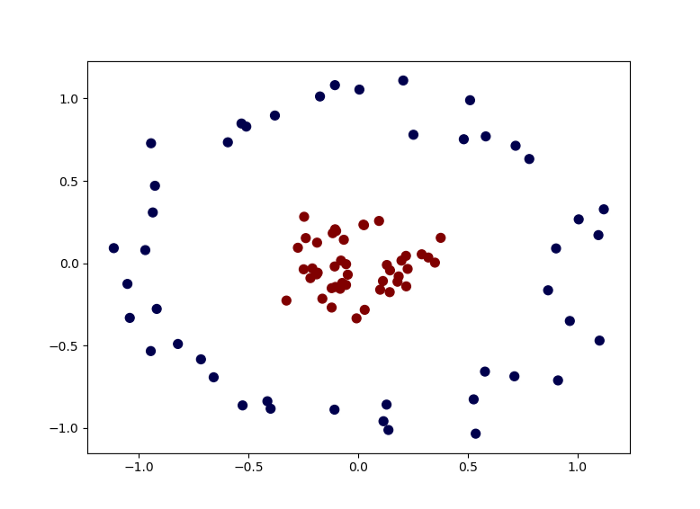
\includegraphics[width=0.7\textwidth]{figures/kernel.png}
	\caption{Example of non separable data.}
	\label{fig:kernel}
\end{figure}

The basic paradigm become:
\begin{itemize}
	\item Given a domain $X$, choose a mapping $\phi : X \rightarrow F$, for some feature space F;
	\item Given a training set $S = ((\mathbf{x}_1, y_1), \dots , (\mathbf{x}_m, y_m))$, apply the mapping to the instances $\hat{S} = ((\phi(\mathbf{x}_1, y_1)), \dots , (\phi(\mathbf{x}_m), y_m))$;
	\item Train a linear predictor $h$ on $\hat{S}$;
	\item New predictions of some point $\mathbf{x}$ are made on $h(\phi (\mathbf{x}))$.
\end{itemize}

An example of solution with kernel is shown in Figure \ref{fig:kernel-3d}, where data are mapped with the function 
\[ \phi : \mathbb{R}^2 \rightarrow \mathbb{R}^3 \]
\[ \mathbf{x} \rightarrow (\mathbf{x}, \left\lVert \mathbf{x} \right\rVert)^2 \]

\begin{figure}[ht]
	\centering
	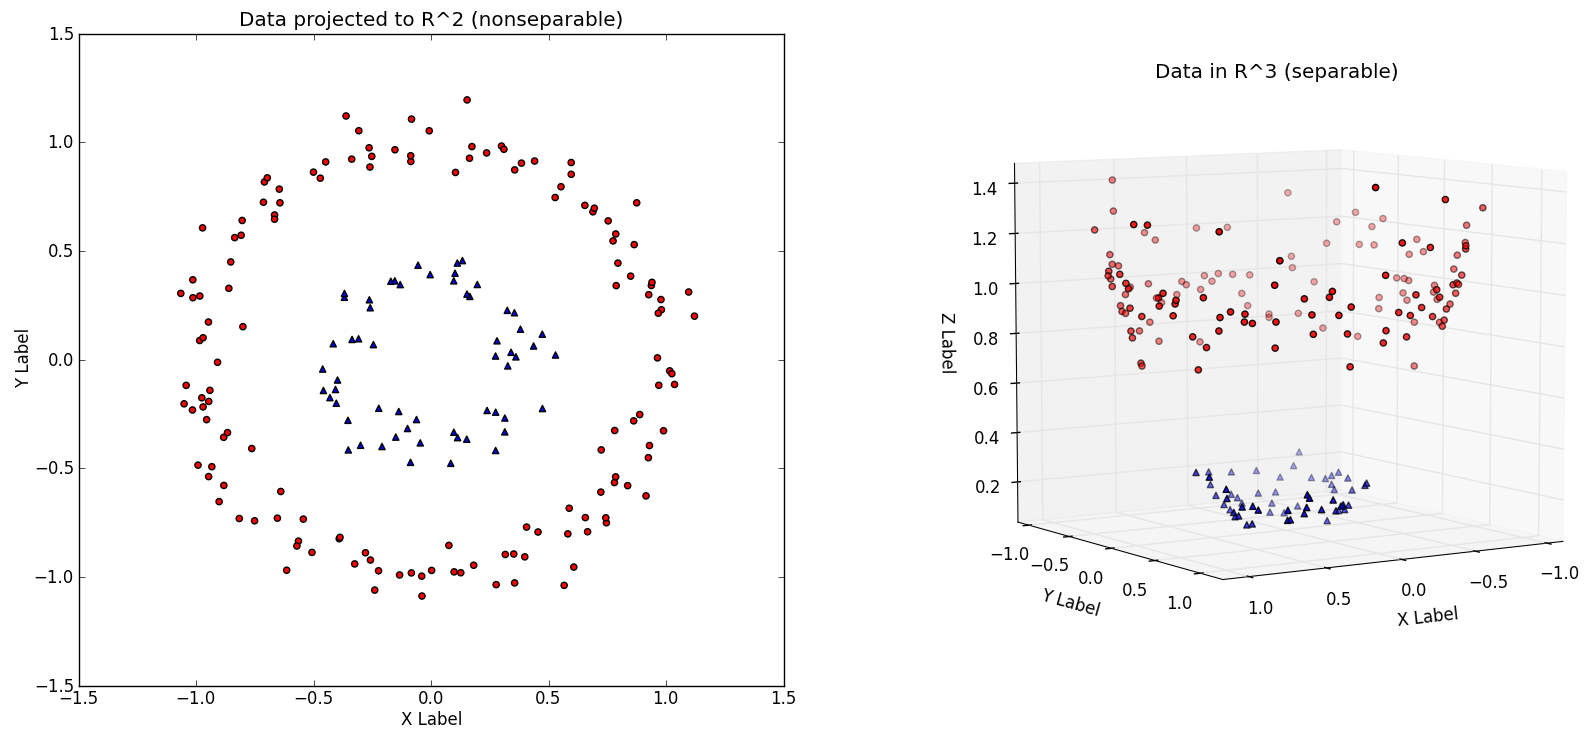
\includegraphics[width=1\textwidth]{figures/kernel-3d.png}
	\caption{Exaxmple of solution with kernel.}
	\label{fig:kernel-3d}
\end{figure}

Embedding the input space into a higher dimensional space, makes the halfspace class more expressive. However, computing the separating hyperplane in a high dimension may be computational expensive. Looking at the SVM dual optimization problem, the increasing computational cost comes from the calculation of $\langle \mathbf{x}, \mathbf{x}' \rangle$, to the calculation of $\langle \phi(\mathbf{x}), \phi(\mathbf{x}') \rangle$ (called also \textit{Kernel Function} $K(\mathbf{x}, \mathbf{x}')$). However, for some kernel functions, it is possible to calculate directly $\langle \phi(\mathbf{x}), \phi(\mathbf{x}') \rangle$ without passing through firstly the calculation of the mapping and then the inner product, that saves some computation. This procedure is called \textit{Kernel Trick}.\\
Some examples of the  most used kernel functions are:
\begin{itemize}
	\item K-degree Polinomial kernel
	\[K(\mathbf{x}, \mathbf{x}') = (1 + \langle \mathbf{x}, \mathbf{x}' \rangle)^k\]
	\item Gaussian kernel 
	\[K(\mathbf{x}, \mathbf{x}') = e^{- \frac{\left\lVert \mathbf{x} - \mathbf{x}' \right\rVert^2}{2 \sigma}} \]
	\item Radial Basis Function (RBF) kernel
	\[K(\mathbf{x}, \mathbf{x}') = e^{- \gamma \left( \mathbf{x} - \mathbf{x}' \right)^2} \]
\end{itemize}
Where $\sigma$ on gaussian kernel, and $\gamma$ on RBF kernel are parameter. is shown in Algorithm \ref{alg:SVM-kernel-SGD}


\subsection{Random Forest}

Recalling that the goal of classification is to minimize a cost function $L_D(h)$ by optimizing the empirical risk $L_s(h)$ (eventually including the regularization term), the so called \textit{Ensemble} models try to obtain the optimal value from a collection of multiple \textit{base learners} $h_1(\mathbf{x}), \dots, h_J(\mathbf{x})$. These learners are then combined to obtain the final prediction $h(\mathbf{x})$ by "voting" the most common outcome.
\[ h(x) = argmax_{y \in \mathcal{Y}} |[j \; for \; j \in [J] \; if \; h_j(\mathbf{x}) = y]| \] 

\textit{Random Forest} is an ensemble learning model, based on \textit{Decision Trees} base learners \cite{inbook}.

\subsubsection{Decision Trees}
A decision tree is a flowchart-like tree structure, where each internal node represent a test on an attribute, each branch represent an outcome of the test, class label is represented by each leaf node \cite{article-decisiontrees}. For instance, suppose we want to predict whether a person is fit, given some simple information like the age, or what he eat. A decision tree that makes that classification may be the one in Figure \ref{fig:decision-tree}.

\begin{figure}[ht]
	\centering
	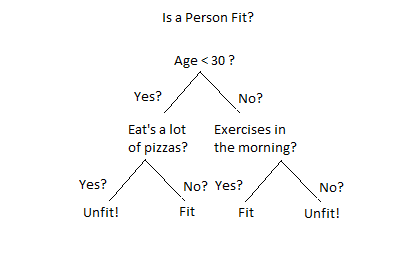
\includegraphics[width=0.7\textwidth]{figures/decision-tree.png}
	\caption{Decision Tree for decide whether a person is fit.}
	\label{fig:decision-tree}
\end{figure}

The task of learning a decision tree consists on determine the splits that define the tree, such that the loss is minimized. Searching for the optimal decision tree that minimizes the loss is computationally hard, so it is preferable to adopt heuristic rules where the tree is built step-by-step by searching a locally optimal solution. \\
A general procedure for building a decision tree starts with a single leaf tree (root), and assigns this node the label according to the majority vote among all labels on the training set. Now, for a series of iterations, it is examined the effect of splitting a single leaf. Defining as \textit{gain} a measure of improvement due to the split, the goal for each step is to find the split that reaches the maximum gain.\\
A possible implementation of decision tree learning algorithm, based on information gain metrics for the splitting criterion, is known as "ID3" (Iterative Dichotomizer 3) \cite{inproceedings-id3}. 





At each iteration, the algorithm selects the attribute with highest information gain as splitting attribute. When information gain approaches to zero, the growing of the tree stops. A recursive solution is shown in Algorithm \ref{alg:ID3}.

\begin{algorithm}
	\caption{ID3(S, A)}
	\label{alg:ID3}
	\begin{algorithmic}[1]
		\State \textbf{input}: training set $S$, feature subset $A \subseteq [d]$
		
		\If{all examples in $S$ are labeled with $1$}
		\State \textbf{return} a leaf $1$
		\EndIf
		\If {all examples in $S$ are labeled with $0$}
		\State \textbf{return} a leaf $0$
		\EndIf
		\If {$A = \emptyset$}
		\State \textbf{return} a leaf whose value = majority of labels in $S$
		\Else
		\State Let $j = argmax_{i \in A} IG(S, i)$
		\If {all examples in $S$ have the same label}
		\State \textbf{return} a leaf whose value = value of the majority of the labels in $S$
		\Else
		\State Let $T_1$ be the tree returned by ID3($\{(\mathbf{x}, y) \in S : S: x_j = 1\}, A \ {j}$)
		\State Let $T_2$ be the tree returned by ID3($\{(\mathbf{x}, y) \in S : S: x_j = 0\}, A \ {j}$)
		\State \textbf{return} left child of the input node = T2, right child of the input node = T1
		\EndIf
		\EndIf

	\end{algorithmic}
\end{algorithm}

A similar approach described in "CART" (Classification and Regression Trees) \cite{cart84}, involves the \textit{Gini} index, instead of information gain. Gini index is calculated as 
\[ Gini = 1 - \sum_{i=1}^{C} (p_i)^2 \]
Where $p_i$ is the probability of a value $i$ in the distribution of the interested attribute. The Gini index is calculated for each attribute, and the split is made with respect to the attribute with lowest value of Gini index.


\subsubsection{Random Forest}
Decision Trees lead easily to overfitting. A solution to prevent the issue, is to construct an ensemble of trees, which is the basic of Random Forest Classifiers. In Rando Forest, each decision tree is constructed by applying the mentioned algorithm on the training set $S$ and an additional randome vector $\Theta$, where $\Theta$ is sampled from some distribution. The final prediction is obtained by the majority of the votes. There are many ways to define the vector $\Theta$, a possible one is the following:
\begin{itemize}
	\item Take a random subsample of $S$, obtaining $S'$;
	\item Construct a sequence $I_1, I_2, \dots$ where each $I_t$ is a subset of $[d]$ of size $k$, generated by sampling $k$ random elements from $[d]$;
\end{itemize}
Finally, each Decision Tree is based on the set $S'$, where at each split, it is restricted to choosing among the set of features $I_t$



\subsection{Na{\"i}ve Bayes}

Na{\"i}ve Bayes is a subset of Bayesian decision theory \cite{Taheri:2013:LNB:3062637.3062651}. It is called na{\"i}ve because the formulation makes some assumptions. The classifier assumes that each feature only depends on the class of the instance (that implies also that all features are independent each other), as shown in Figure \ref{fig:naive-bayes}. However, in real world cases, it is not possible to guarantee this assumption, but the classifier works still reaches good results.\\

\begin{figure}[ht]
	\centering
	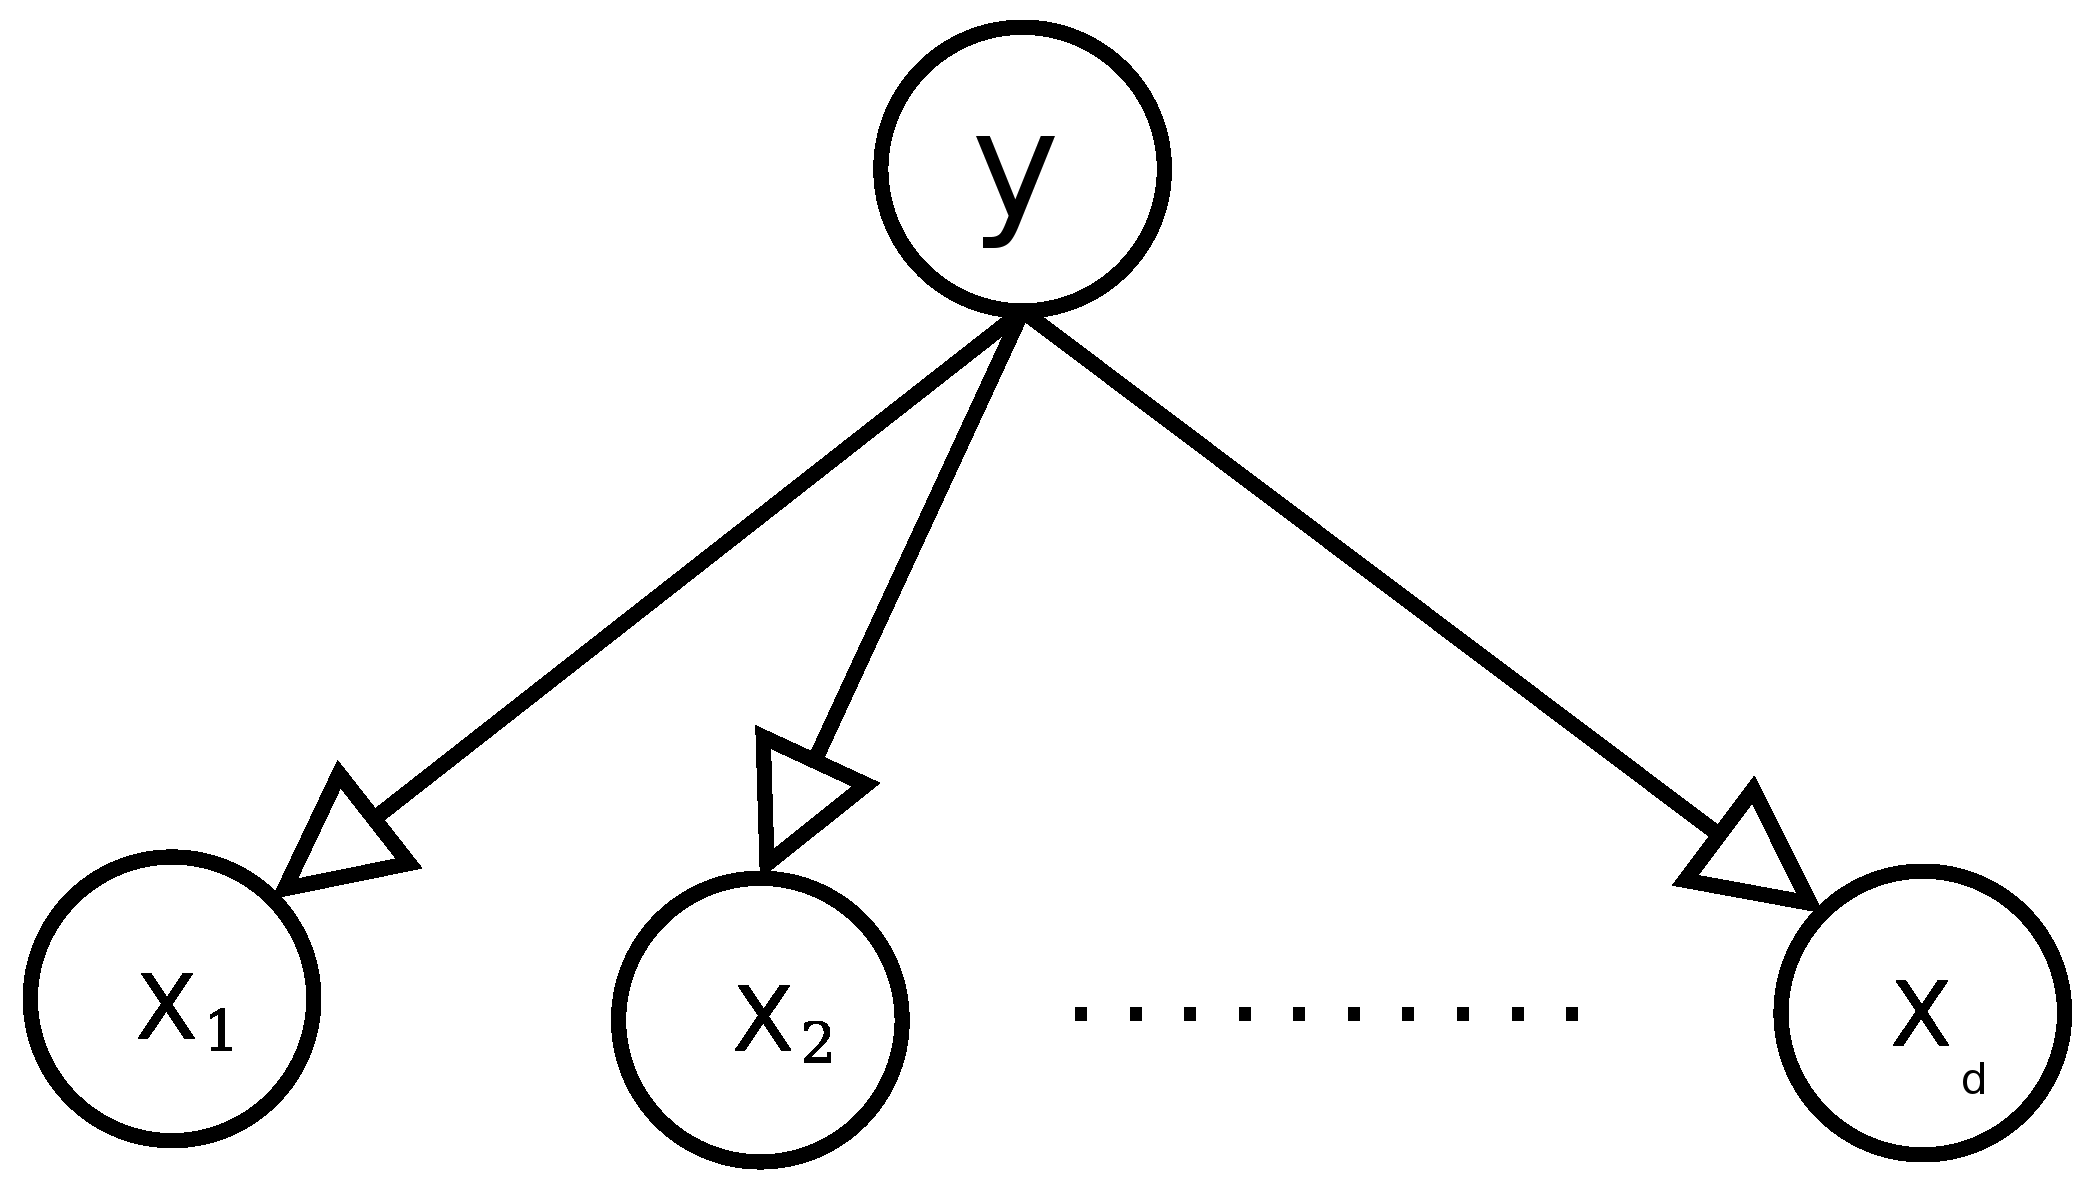
\includegraphics[width=0.7\textwidth]{figures/naive-bayes.png}
	\caption{Features independency on Na{\"i}ve Bayes classifier.}
	\label{fig:naive-bayes}
\end{figure}

Let $y$ denote the class of an observation $\mathbf{x}$. Predict the class of $\mathbf{x}$ by searching the class $y$ that maximize the value of the Bayes Rule (posterior probability)
\[ \mathbb{P}(y | \mathbf{x}) = \frac{\mathbb{P}(y)\mathbb{P}(\mathbf{x} | y)}{\mathbb{P}(\mathbf{x})} \]
Exploiting  the fact that the features $x_1, \dots, x_d$ are independent, the following equation is sufficient to predict the most probable class
\[ \mathbb{P}(y | \mathbf{x}) = \frac{\mathbb{P}(y)\prod_{i=1}^{d}\mathbb{P}(x_i | y) }{\mathbb{P}(\mathbf{x})} \]





\subsection{Multiclass Classification}

Since this point, all classification algorithms are thought for binary classification, namely for a labels set $\mathcal{Y}={-1, +1}$. However, many real world classification problems require a larger labels set, leading to a multiclass classification problem. Some algorithms, thought for binary classification, can be extended in the multiclass case, for instance Na{\"i}ve Bayes and Support Vector Machines, while other approaches convert the multiclass problem into a set of binary ones that are solves using common classification algorithms \cite{Aly05surveyon}. Two main approaches belonging to the second category are the so called \textit{One-Versus-One} (OVO) and the \textit{One-Versus-Rest} (OVR). Below are explained some methods for multiclass classification, that have been used in this work.

\subsubsection{Multiclass Classification for Na{\"i}ve Bayes}

Na{\"i}ve Bayes classifier works actually in multiclass case. Given a problem with $k$ classes $(y_1, \dots, y_k)$, it assigns the label $y$ to an unknown example $\mathbf{x} = (x_1, \dots, x_d)$ by maximizing the posterior probability, formally
\[ y = argmax_{y \in (y_1, \dots, y_k)} \mathbb{P}(y | x_1, \dots, x_d)  \]
That works independently on 2-labels classes or 3+ labels classes.

\subsubsection{One-Versus-All}
The simplest approach is to reduce the problem of classifying among $k$ classes into $k$ binary problems, where each problem discriminates a given class from the other $k-1$. For this approach, are needed $k$ different classifiers. For each class, it is trained a binary classifier with the entire training set, where positive samples are the one belonging to that class, while the negative ones are all the others. This approach is summarized in Algorithm \ref{alg:OVA}.

\algnewcommand\algorithmicforeach{\textbf{for each}}
\algdef{S}[FOR]{ForEach}[1]{\algorithmicforeach\ #1\ \algorithmicdo}

\begin{algorithm}
	\caption{One-Versus-All}
	\label{alg:OVA}
	\begin{algorithmic}[1]
		\State \textbf{input}: 
		\State \hskip 1.5em training set $\mathcal{S}=((\mathbf{x}_1, y_1), \dots, (\mathbf{x}_n, y_n))$
		\State \hskip 1.5em algorithm for binary classification A
		
		\ForEach {$i \in \mathcal \mathcal{Y} $}
		\State let $S_i = ((\mathbf{w}_1, (-1)^{y_i \neq i}), \dots, (\mathbf{w}_n, (-1)^{y_i \neq i}))$
		\State let $h_i = A(S_i)$
		\EndFor
		
		\State \textbf{output}:
		\State \hskip 1.5em the multiclass hypothesis defined by $h(\mathbf{x}) = argmax_{i \in \mathcal{Y}} h_i(\mathbf{x}))$
		
		
	\end{algorithmic}
\end{algorithm}


\subsubsection{One-Versus-One}

In this approach, each class is compared to each other class. For each pair of classes, a binary classifier is built to discriminate between them, and ignoring all others. Saying $k$ the total number of classes, this method require $\binom{k}{2} = \frac{k(k-1)}{2}$ total binary classifiers. When voting a new instance, it is performed a voting for each classifier, and the class with maximum number of votes is the actual one. This approach is summarized in Algorithm \ref{alg:OVO}.

\begin{algorithm}
	\caption{One-Versus-One}
	\label{alg:OVO}
	\begin{algorithmic}[1]
		\State \textbf{input}: 
		\State \hskip 1.5em training set $\mathcal{S}=((\mathbf{x}_1, y_1), \dots, (\mathbf{x}_n, y_n))$
		\State \hskip 1.5em algorithm for binary classification A
		
		\ForEach {$i, j \in \mathcal \mathcal{Y}, i < j $}
		\State initialize $S_{i,j}$ to be an empty sequence
		\For $t=1, \dots, m$
		\State \textbf{if} $y_t = i$ add $(\mathbf{x}_t, 1)$ to $S_{i,j}$
		\State \textbf{if} $y_t = j$ add $(\mathbf{x}_t, -1)$ to $S_{i,j}$
		\EndFor
		\State let $h_{i,j} = A(S_{i,j})$
		\EndFor
		
		\State \textbf{output}:
		\State \hskip 1.5em $h(\mathbf{x}) \in argmax_{i \in \mathcal{Y}} \left( \sum_{j \in \mathcal{Y}} sign(j-i) h_{i,j}(\mathbf{x}) \right)$
		
		
	\end{algorithmic}
\end{algorithm}



\subsection{Classification Metrics}

Machine learning classification performance is related to state how well a classifier, that implements a specific machine learning algorithm, makes a correct discrimination between classes. The most basic stated problem consists in binary classification, so most of the metrics are based on this task, and then extended to multiclass problems.\\
It is important to introduce some terminology about the four types of direct results in binary classification, namely \textit{True Positives} (TP), \textit{True Negatives} (TN), \textit{False Positives} (FP), \textit{False Negatives} (FN) \cite{inproceedings-bin-metrics}. These values are commonly displayed in 2 rows by 2 columns of the so called \textit{confusion matrix}, as shown in Figure \ref{fig:confusion-matrix}. 

\begin{figure}[ht]
	\centering
	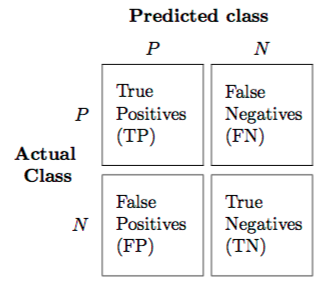
\includegraphics[width=0.6\textwidth]{figures/confusion_matrix.png}
	\caption{Confusion matrix for binary classification metrics.}
	\label{fig:confusion-matrix}
\end{figure}

These four direct outputs of the classifier are also called "base measures", and the meaning is the following: "True" classification results (TP and TN) are the instances that the classifier discriminated correctly, and are located in the diagonal of the confusion matrix, whereas "False" classification results (FP and FN) are the mistakes of the classifier and are displayed in off-diagonal of the confusion matrix. False Positives instances consist on instances that are classified as "positive", but the correct label was "negative", while False Negatives samples consist on in instances that are classified as "negative", but the correct label was "positive". For what seen, it is mandatory to define a "positive" class for measuring a classification metrics on a real world problem, and it depend on the goal of the task.\\
In some problems, False Negatives could be more serious than False Positives, for instance in medical fields it means that a disease is not recognized. In this case it is better to classify positively a disease that is not "malign", instead of ignore it. \\
In the following sections, are explained some performance metrics, derived from the base measures, that have been exploited in this work.

\begin{itemize}
	\item \textit{Accuracy} is the ratio of total number of correctly classified instances, over the size of the sample set, formally
	\[ Accuracy = \frac{TP + TN}{TP + TN + FP + FN} \]
	It is the most provided, and the most abused metric in binary classification. Using accuracy as a benchmark measurement has some limitations, in fact it can lead to suboptimal solutions, especially when dealing to imbalance class distributions. Another limitation pf accuracy is that it prodices less distinctive and less discriminable values, consequently it leads to less discriminating power to accuracy in selecting the optimal classifier. In addition, accuracy also lacks in informativeness about minority class instances \cite{article-ev-metrics}.
	
	\item \textit{Precision} is used to measure the positive instances that are correctly classified from the total predicted ones in positive class, formally
	\[ Precision = \frac{TP}{TP + FP} \]
	
	\item \textit{Recall} is used to measure the fraction of positive samples that are correctly classified, formally
	\[ Recall = \frac{TP}{TP + FN} \]
	
	\item \textit{F-Score} represent the harmonic mean between precision and recall, formally
	\[ F-score = \frac{2 \times precision \times recall}{precision + recall} \]
\end{itemize}

To generalize the presented classification metrics from binary to multiclass there are two average methods. Saying $\mathcal{Y}={y_j : j = 1, \dots, q}$ the list of all possible labels, $EM(TP, TN, FP, FN)$ an evaluation metric that is calculated on the number of TP, TN, FP, FN, $tp_y$, $tn_y$, $fp_y$, $fn_y$ the number of classification results with respect to a label $y$, the average metrics are:

\begin{itemize}
	\item The \textit{macro-average} is calculated as
	\[ EM_{macro} = \frac{1}{q} \sum_{y \in \mathcal{Y}} EM(tp_y, tn_y, fp_y, fn_y) \]
	
	\item The \textit{micro-average} is calculated as
	\[ EM_{micro} = EM \left( \sum_{y \in \mathcal{Y}} tp_y, \sum_{y \in \mathcal{Y}} tn_y, \sum_{y \in \mathcal{Y}} fp_y, \sum_{y \in \mathcal{Y}} fn_y,  \right) \]
\end{itemize}

There is no rule about what average score is better. Micro-averaged score may be misleading, because more frequent labels are weighted heavier, and thus in favor of macro-averaged, but in the same way, sometimes it is needed that labels need to be counted proportionally with their influence, so preferring micro-averaged. It depends on the application.



\section{Sentiment Analysis Algorithms}

Sentiment Analysis is a widely studied field of Natural Language Processing, so many algorithms have been proposed in order to achieve the best performance possible. However, the algorithms usually are focused in one type of documents (mostly Twitter's comments), and sometimes in one domain of interest, for instance pharmaceutical.\\
In this section a sentiment analysis algorithm, that has been taken in some parts for this work, is presented, along with some other works in contest of forum sentiment analysis.


\subsection{BPEF}

\textit{Bootstrap Ensemble Framework} (BPEF) \cite{Hassan2013TwitterSA} is a text mining framework for Twitter Sentiment Analysis. It is thought to overcome some well known issues on TSA, which are high class imbalance and representational richness issues. In \cite{Zimbra:2018:STS:3210372.3185045} it is shown that in experimental results this approach reaches the best performance in its prediction across sentiment classes, as compared to various comparison tools and algorithms. Consequently, BPEF is able to build strong class predictions, from here the choice of implementing some of its parts for this work. In Figure \ref{fig:bpef} the whole procedure of BPEF is summarized.\\
\\
BPEF is essentially a two-stages process that includes an expansion stages, followed by a contraction stage. By parametrizing the learning procedure, it has been possible to generate a large, diverse set of learned models, that is the expansion stage. After that, the contraction is performed, that is essentially the search of the optimal subset of produced models, which when voted in an ensemble, maximize the overall performance.\\
\\
As shown in Figure \ref{fig:bpef}, expansion is made for three components: datasets, feature and models. At each component, are introduced some parameters which when changed produce newer models. In the following paragraphs are explained the parameters.

\subsubsection{Dataset Parameters}

In addition to the target dataset (the one of interest), some other dataset have been used. It has been produced a category of parameters responsible to mix the additional datasets with the one of interest. By choosing a different combination of datasets it is possible to create a new training dataset which is used to train different models. Datasets have been chosen from similar fields, for instance consumer product reviews. By mixing diverse datasets, it is expanded the number or patterns used to express sentiment polarities, by including instances from different sub-domains. The models learned on instances from mixture of datasets are intended to learn general or subdomain independent sentiment patterns.

\subsubsection{Feature Parameters}

Different feature types have been adopted as parameter category. Both basic feature types and more generalizing feature variations (used to decrease sparsity on data) have been used as feature parameters.\\
Feature types consist of unigrams and bigrams of
\begin{itemize}
	\item Simple words;
	\item Parts-Of-Speech;
	\item Parts-Of-Speech and words combined;
	\item SentiWordNet features (SWNt), from the need to represent subjective words used scarcely, that may be dropped out during feature selection phase. These words are replaced with their sentiment polarity derived using the SentiWordNet lexical resource \cite{Esuli2006sentiwordnet}. SENt features are represented as "POS-X", "NEG-X" and "NEU-X", incorporating positive, negative or neutral polarity, where "X" is a positive integer proportional to the strength of the sentiment according to the score derived by aggregating polarity scores across word senses;
	\item Semantic features (Synset tags derived using WordNet);
\end{itemize}

On top of these four basic feature groups, it has been applied a feature summarizing technique, like Legomena (replacing once occurring word with a tag) and Named Entity Recognition (NER), in order to reduce sparsity on data.

\subsubsection{Classifier Parameters}

BPEF includes in its learning stack different classification algorithms commonly used in prior text classification and sentiment analysis algorithms. \\

\begin{figure}[ht]
	\centering
	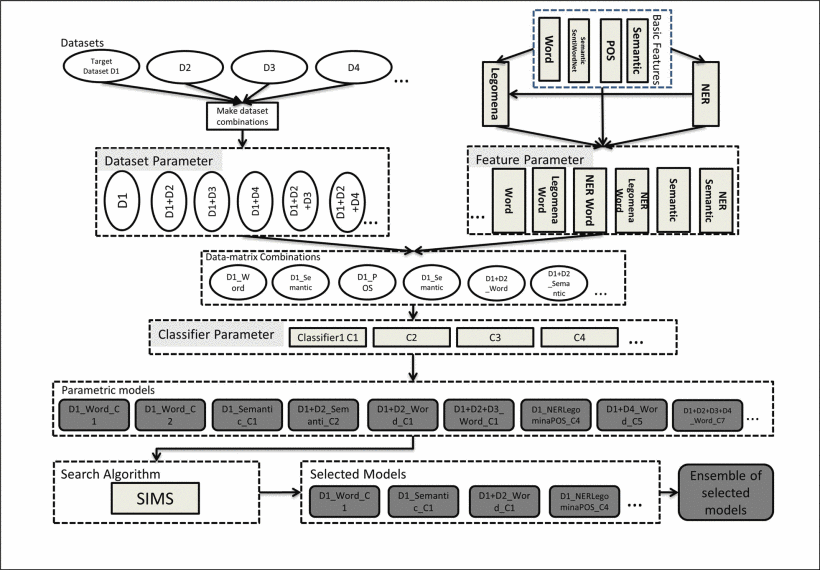
\includegraphics[width=1\textwidth]{figures/bpef.png}
	\caption{Diagram that summarize the BPEF procedure.}
	\label{fig:bpef}
\end{figure}

 As shown in Figure \ref{fig:bpef}, each combination of dataset, feature and classifier, define a new model, so the total learned models are the product of the number of datasets, feature sets and classifiers.\\
 All these models are trained using \textit{bootstrap samples}, which are balanced subsamples of the training set. This solution may overcome the imbalances issues characteristics of TSA.
 
 
 \subsubsection{Contraction: Step-Wise Model Selection}
 In expansion stage, a large number of model are generated, while in contraction stage the goal is to improve the performance of the ensemble by keeping only a subset of the total models, in order to remove redundancy and less useful models. Since there are $2^p$ possible combination of $p$ parametric models, exhaustive search strategies are infeasible. For this reason, it is proposed a Step-wise Iterative Model Selection (SIMS) approach, which is based on a greedy search, that is more efficient even if it does not guarantee to find the optimal solution.\\
 SIMS is a 2 steps hierarchical application of the IMS subroutine. First, IMS is applied on each bootstrap model (which actually is a combination of three binary classifier: Pos-Neu, Pos-Neg, Neu-Neg). IMS (Algorithm \ref{alg:IMS}) is used to select a subset of binary classifiers associated to the $n$ bootstrap models comprising $3n$ total binary classifiers. Next, IMS is applied directly on the set of parametric models. The greedy approach searches, at each iteration, the model that gives the best result when combined with the already selected ones. The final SIMS pseudocode is shown in Algorithm \ref{alg:SIMS}.
 
  \begin{algorithm}
 	\caption{IMS}
 	\label{alg:IMS}
 	\begin{algorithmic}[1]
 		
 		\State $modelsSelected = []$
 		\State $parametricModels = [model1, model2, ...]$
 		\State 
 		\State \textbf{input}: $models$, $modelsSelected$
 		
 		\State $maxaccuracy = 0$
 		\State \textbf{repeat} until $models$ is empty:
 		\State \hskip 1.5em $x = argmax_{X \in models}(accuracy(X + modelsSelected))$
 		\State \hskip 1.5em $accX = accuracy(X + modelsSelected)$
 		\If $accX > maxaccuracy$
 		\State $maxaccyracy = accX$
 		\State $modelsSelected = modelsSelected + x$
 		\State $models.pop(x)$
 		\EndIf
 		\Return $modelsSelected$
 		
 	\end{algorithmic}
 \end{algorithm}
 
\begin{algorithm}
	\caption{SIMS}
	\label{alg:SIMS}
	\begin{algorithmic}[1]
		
		\State $combPerf = []$
		\State $binComb = $ 3 tuple combination of binary models
		\State  
		\For $B1, B2, B3$ in $BinComb$
		\State $B1Models = $ IMS($B1, []$)
		\State $B21Models = $ IMS($B1, B1Models$)
		\State $B321Models = $ IMS($B1, B21Models$)
		\State $combPerf$.append($B321$)
		\EndFor
		\State $chosenComb = argmax_{X \in combPerf}$accuracy($X$)
		\State IMS($chosenComb, []$)
		
	\end{algorithmic}
\end{algorithm}

\subsubsection{Results}

In \cite{Hassan2013TwitterSA}, BPEF has been compared with other sentiment analysis tools with respect to recall and accuracy metrics. The final results show that BPEF outperforms the comparison models by a wide margin (16\% to 20\% higher recall), and also reaches balanced performance across all classes.\\
It has also been shown the additive contribution of the three component parameters: the study consisted in removing, one at time, all parameters and compared the performance against the SIMS applied on all parametric models. For instance, in order to evaluate the effectiveness of the dataset parameters, those are excluded. The results show that the greatest impact comes from the classifiers parameters, while features parameters have just a shallow impact on the overall performance.


\subsection{Related Works}

Sentiment analysis have been utilized in multiple fields in order to investigate people's opinion. In \cite{ali-etal-2013-hear}, sentiment analysis has been applied in the medical field, in order to obtain relations between positive and negative opinions and patients' health, more precisely on hearing loss. The study had two stages: the first consisted on manual annotation of web forums' comment, and the last was the actual classification adopting machine learning techniques. The retrieved dataset consisted in 3515 sentences from 26 threads, that have been extracted from 607 individual posts using regular expression tools. Then, the sentences have been annotated in the three degrees of polarity "positive", "neutral" / "unknown" and "negative" by two manual annotators. All the sentences that did not contain sentiment information have been removed, in fact most of the sentences have been actually discarded, but considering just interested ones, classes resulted balanced, reducing biases to the classifier. It has been also considered the quality of the classification by look for a score that evaluated the agreement of the two annotators, which gives good results, so data may be considered reliable. Classification involves, along with Bag of Words, other few features extracted from each sentence, that are the number of: words with strong subjective (involving a resource like SentiWordNet), words with weak subjective, adjectives, adverbs, pronouns, words having positive, negative and neutral polarities, phrases containing pronouns. Final classification experiments involved machine learning algorithms such as Na{\"i}ve Bayes, SVM and Logistic Regression. Final results show the best F-score obtained in multiple experiments of 0.685, reached using the Logistic Regression classifier.









